\chapter{Stokastiske variable}
\label{kap:stokastiske} % Opprinnelig kapittelnr: 5

\section{Innledende definisjoner}

La utgangspunktet være et eksperiment med et gitt utfallsrom.
\footnote{I dette kapitlet kommer en mengde nye begreper, som det ikke
alltid er like lett å motivere, fruktene kommer senere.
Det er ikke vanskelig, men det krever konsentrasjon: Lukk døra, slå av
CD-spilleren og stump røyken!}
Formålet med observasjon  behøver ikke nødvendigvis være å
få vite akkurat hvilket av de mulige utfall som inntreffer.
For mange problemstillinger er en mindre
detaljrik beskrivelse av eksperiment\-resultatet tilstrekkelig.
Ofte er det bekvemt med en tallmessig beskri\-velse, dvs. vi er
interessert i en tallstørrelse som er entydig gitt ved utfallet
av eksperimentet, og som delvis karakteriserer dette, eksempelvis

\begin{itemize}
\item  I to terningkast kan det hende at vi bare er interessert i
   summen av øynene, og ikke resultatet av hvert enkelt kast.
\item  I kvalitetskontroll er vi ofte interessert i antall defekte
   artikler i et utvalg, ikke hvilke artikler som var defekte
   eller ikke.
\item  I en binomisk forsøksrekke er vi som oftest interessert i
   antall suksesser, ikke hvilke forsøk som ga henholdsvis
   suksess og fiasko.
\end{itemize}

\noindent Ved å trekke ut slike tallstørrelser kan vi ofte bearbeide
eksperimentresultatet på en mer hensiktsmessig måte.

\begin{center} \framebox[10cm]{\begin{minipage}{9cm}\rule{0cm}{0.5cm}
   \begin{definisjon}
     Gitt et eksperiment med utfallsrom $\Omega$.\\
     En {\em stokastisk variabel} er en funksjon med utfallsrommet
     $\Omega$ som definisjonsmengde og verdimengde blant reelle tall R.
   \end{definisjon}
  \end{minipage}} \end{center}

\noindent Stokastiske variable betegnes som oftest med store bokstaver fra
slutten av alfabetet f.eks. $X$, $Y$, $Z$, $U$, $V$, $W$ etc. 
\footnote{I moderne matematikk er det ikke god tone å kalle en funksjon
for en variabel, men det er uhensiktsmessig å endre en allerede
innarbeidet notasjon på dette punkt.}) La $X$ være en stokastisk
variabel (s.v.). $X$ er da en forskrift som til ethvert utfall
$u$ i utfallsrommet tilordner et reellt tall $X(u)$:

\[         X : u \rightarrow X (u)\]

\begin{eksempel}{To myntkast}
Anta at utfallsrommet er $\Omega$ = \{MM, MK, KM, KK\}.
La $X$ være en stokastisk variabel definert ved
 \begin{center}
  \begin{tabular}{cccccc}
            $u$ & : & MM   & MK   & KM   & KK \\
          $X(u)$& : &   0  &  1   &   1  &  2
  \end{tabular}
\end{center}

\noindent Vi ser at $X$ representerer antall kron i de to kastene. Den
stokastiske variable $X$ er illustrert i Figur~\ref{fig:stokastisk_variabel}.
\end{eksempel}

\begin{figure}[ht]
\centering
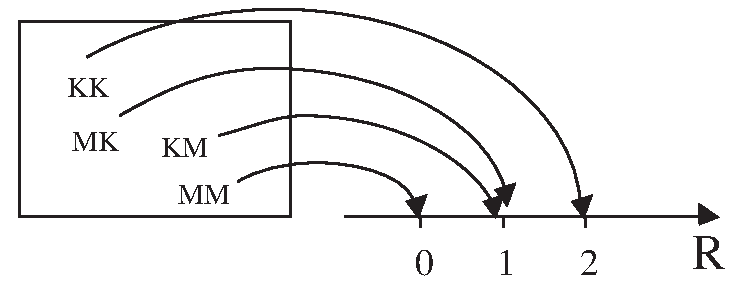
\includegraphics[scale=0.8]{figurer/fig5_1.pdf} 
\caption{En stokastisk variabel}
	\label{fig:stokastisk_variabel}
\end{figure}

\begin{eksempel}{To terningkast}
Anta at utfallsrommet er $\Omega = \{(1,1), (1,2),...,(6,6)\}$.
La $S$ være en stokastisk variabel definert ved

\[   S((1,1))=2, \;  S((1,2))=3, \; \ldots, \; S((6,6))=12 \]

\noindent dvs. til utfallet $(i,j)$ tilordnes det reelle tallet $i+j$. Vi ser
at $S$ representerer summen av øynene i de to kastene.
\end{eksempel}

\begin{eksempel}{Tombola}
I en tombola er det N lodd nummererte fra 1 til N.
Et lodd trekkes tilfeldig, og trekkes lodd nr. $i$ får man en
gevinst av verdi $v_i$ (som kan være positiv, null eller
negativ). La utfallsrommet være $\Omega = \{1,2,...,N\}$, og la
$Y$ være den stokastiske variabel som til utfallet $i$ tilordner
verdien $v_i$. Vi ser at $Y$ representerer verdien av det
uttrukne lodd.
\end{eksempel}

\begin{eksempel}{Indikator}
La $A$ være en begivenhet i et utfallsrom $\Omega$.
Dersom $X$ er en stokastisk variabel definert ved at
\[   X(u)= \left\{ \begin{array}{ll}
    1 & \mbox{for alle  $u \in A$} \\
    0 & \mbox{for alle $ u \in \bar{A}$}
            \end{array} \right. \]
\noindent sier vi at $X$ er en {\em indikatorvariabel}, den indikerer om
begivenheten $A$ har inntruffet eller ikke.
\end{eksempel}

\begin{eksempel}{Ventetid til første kron}
Anta at vi har valgt $\Omega$ = \{K, MK, MMK, MMMK,\ldots\} som
utfallsrom. La $N$ være en stokastisk variabel definert ved
\begin{center}
 \begin{tabular}{ccccccc}
            $u$ & : & K & MK & MMK & MMMK & \ldots \\
         $N(u)$ & : & 1 & 2  &  3  &  4   & \ldots
 \end{tabular}
\end{center}
Da vil $N$ representere ventetiden til første kron.
\end{eksempel}

I anvendelser hvor utfallsrommet selv er en delmengde av de
reelle tall, kan det komme på tale å bruke identitetsfunksjonen
som stokastisk variabel, dvs. definere $X$ ved

\[  X(u) = u \mbox{\ \ for alle  } u \in \Omega \]

\noindent eksempelvis vil $X=$ antall øyne i et terningkast kunne
oppfattes som den stokastiske variable som til utfallet ``i øyne''
tilordner det reelle tall $i$.


\section{Sannsynlighetsfordeling}

La $X$ være en stokastisk variabel definert i et utfallsrom
$\Omega$. Med symbolkombinasjonen $(X=x)$ vil vi forstå den
begivenhet at den stokastiske variable $X$ antar verdien $x$,
eller presist

\[ (X=x)=\{u; X(u)=x\} \]

\noindent dvs. gunstige utfall for begivenheten $(X=x)$ er de utfall $u$
som er slik at $X(u)=x$. La oss betegne de mulige 
 \footnote{For enkelhets skyld antar vi bare et endelig antall mulige
verdier. Dette vil vi ofte gjøre i det følgende uten at dette er
nødvendig, resultatene gjelder også med visse reservasjoner
dersom vi har et tellbart uendelig antall mulige verdier.}
verdiene av $X$ med $x_1, x_2, ..., x_r$.
Vi vil ofte være interessert i sannsynlighetene for de $r$ begivenhetene

\[           (X=x_1), (X=x_2), \ldots , (X=x_r) \]

\noindent I denne forbindelse innfører vi følgende begrep:

\begin{center} \framebox[10cm]{\begin{minipage}{9cm}\rule{0cm}{0.5cm}
   \begin{definisjon}
     {\em Sannsynlighetsfordelingen} til $X$ er en \\
      oppregning av de mulige verdier av $X$ sammen med
     sannsynligheten for at $X$ antar disse verdiene.
   \end{definisjon}
  \end{minipage}} \end{center}

\noindent Sannsynlighetsfordelingen kan gis i tabellform slik
 \[ \begin{array}{c|cccc}
 x    &   x_1  &   x_2  &\cdots &  x_r \\ \hline
P(X=x)&P(X=x_1)&P(X=x_2)&\cdots &P(X=x_r)
\end{array} \]

\noindent eller ved en funksjon $p$ definert for de mulige verdier av $X$
slik at

\[            p(x)=P(X=x)   \]

\noindent Vi sier at $p$ er {\em (punkt)fordelingsfunksjonen} til $X$.\\

\begin{eksempel}{To myntkast}
Dersom $X=$ antall kron, får vi

\[     (X=0)=\{MM\}, \;\; (X=1)=\{KM,MK\}, \;\; (X=2)=\{KK\} \]

\noindent I en modell hvor alle 4 utfall er like sannsynlige blir
sannsynlighetsfordelingen til $X$
%\begin{center}
 \begin{tabular}{c|ccc}
 $x$    &   0  &   1  &  2 \\ \hline
 $P(X=x)$&$\frac{1}{4}$&$\frac{1}{2}$&$\frac{1}{4}$
\end{tabular}
%\end{center}
\end{eksempel}

\begin{eksempel}{To terningkast}
Dersom $S=$ sum øyne i de to kastene får vi

\[ (S=2)=\{(1,1)\},\; (S=3)=\{(1,2), (2,1)\}, \ldots , (S=12)=\{(6,6)\} \]

\noindent I en modell hvor alle 36 mulige utfall er like sannsynlige blir
sannsynlighetsfordelingen til $S$
\begin{displaymath}\small
\begin{array}{c|ccccccccccc} 
 s   &  2  &  3  &  4  &  5  &  6  &  7  &  8 & 9 & 10  &  11 & 12 \\ \hline
P(S=s)&\frac{1}{36}&\frac{2}{36}&\frac{3}{36}&\frac{4}{36}&\frac{5}{36}&
  \frac{6}{36}&\frac{5}{36}&\frac{4}{36}&\frac{3}{36}&\frac{2}{36}&\frac{1}{36}
  \end{array}
  \end{displaymath}
\end{eksempel}

\noindent Vi merker oss at

\[      \Omega = (X=x_1) \cup (X=x_2) \cup \cdots \cup (X=x_r) \]

\noindent er en disjunkt union. Følgelig blir

 \[      1=P(\Omega )=P(X=x_1)+P(X=x_2)+\cdots +P(X=x_r) \]

\noindent Fordelingsfunksjonen $p(x)$ til $X$ har derfor følgende
egenskaper
\begin{center}
 1. \mbox{\ \ \ }   $0 \leq p(x) \leq 1$ for alle $x$ \\
 2. \mbox{\ \ \ }   $p(x_1)+p(x_2)+ \cdots +p(x_r)=1$
\end{center}
\noindent Vi ser at dette stemmer i Eksempel 6 og 7. \\

\noindent {\bf Merknad}. Ut fra en gitt sannsynlighetsmodell definerer den
stokastiske variable $X$ en ny sannsynlighetsmodell med mengden
av de mulige verdier av $X$ som utfallsrom, dvs. et utfallsrom
bestående av reelle tall

\[ \Omega _X =\{x_1, x_2, ..., x_r\} \]

\noindent og sannsynlighetsfunksjon lik fordelingsfunksjonen $p(x)$ til $X$.\\

Dersom man ønsker å billedliggjøre sannsynlighetsfordelingen til
$X$ tegner man ofte et såkalt {\em histogram}. Dette er en figur
bestående av søyler som hver er sentrert i en mulig verdi av $X$
med areal som er proporsjonalt med sannsynligheten for at X antar denne
 verdien. I eksemplet med to terningkast vil
histogrammet til sum øyne $S$ se ut som i Figur~\ref{fig:histogram_k5}.

\begin{figure}[ht]
\centering
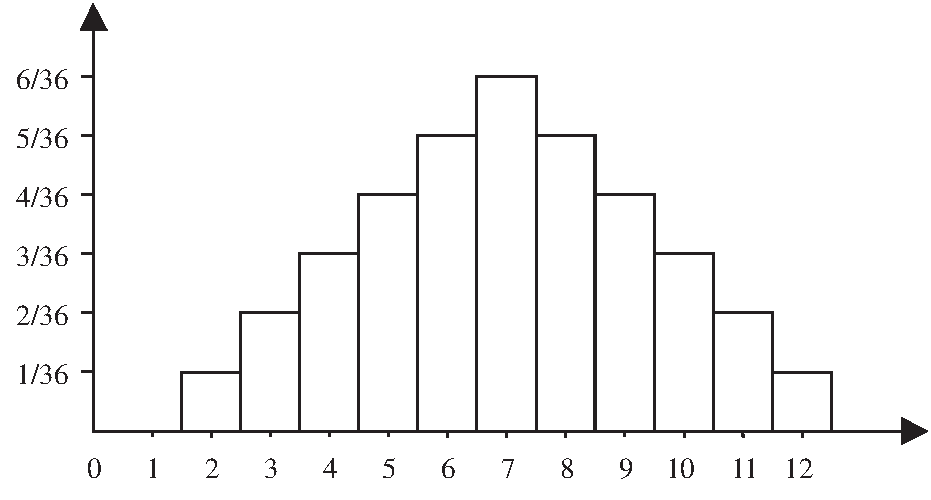
\includegraphics[scale=0.7]{figurer/fig5_2.pdf} 
\caption{Et histogram}
	\label{fig:histogram_k5}
\end{figure}

I mange situasjoner der man er interessert i en stokastisk
variabel $X$, er sannsynlighetsfordelingen $p(x)$ helt eller
delvis ukjent. For å skaffe informasjon om $p(x)$ kan det være
aktuelt å utføre det eksperimentet som modellen er ment å
beskrive gjentatte ganger, og observere verdien av $X$ hver gang.
Vi teller deretter opp antall ganger vi observerte de ulike
mulige verdier av $X$, og tegner en figur med søyler som hver er
sentrert i en mulig verdi av $X$, med areal proporsjonalt med
antall ganger $X$ har antatt denne verdi. En slik figur kalles et
{\em empirisk histogram}. Et empirisk histogram gir oss
informasjon om formen på den sannsynlighetsfordelingen $p(x)$
(dvs. om histogrammet) som svarer til en noenlunde realistisk
modell for eksperimentet. Påliteligheten av denne informasjon vil
selvsagt avhenge av hvor mange ganger vi gjentar eksperimentet,
jfr. tanken om sannsynlighet som idealisert hyppighet i det lange
løp (se Oppgave~42 og Eksempel 1.6).

La $X$ være stokastisk variabel. Det er da naturlig å innføre
følgende skrivemåter

\[ (X \leq x)=\{u;X(u) \leq x\}, \; \; (X>x)=\{u;X(u)>x\}  \mbox{\ \ etc.} \]

\noindent dvs. $(X \leq x)$ betyr begivenheten at $X$ antar en verdi
mindre enn eller lik $x$, mens $(X>x)$ betyr begivenheten at $X$
antar en verdi større enn $x$ etc. Anta at sannsynlighetsfordelingen
til $X$ er gitt ved fordelingsfunksjonen $p(x)=P(X=x)$.
Sannsynligheten for begivenheten $(X \leq x)$ blir lik

\[ F(x)=P(X \leq x)=\sum_{k \leq x}p(k) \]

\noindent dvs. vi summerer sannsynlighetene $P(X=k)$ for alle $k$ som er
$\leq x$. Funksjonen $F(x)=P(X \leq x)$ definert for alle reelle
$x$ kalles den {\em kumulative fordelingsfunksjonen} til $X$.
En kumulativ fordelingsfunksjon $F(x)$ har generelt egenskapene
(i) $F(x)$ ikke avtagende (ii) $0\leq F(x)\leq 1$ 
(iii) $F(-\infty)=0,$ \ $F(\infty)=1$.
For diskrete modeller som vi studerer her, vil den
være en trappefunksjon med sprang i hver av de mulige verdier av
$X$ og trinnhøyde lik sannsynligheten for at $X$ antar verdien,
se Oppgave~38.

Sannsynlighetsfordelingen til $X$ kan alternativt beskrives ved å
angi den kumulative fordeelingsfunksjon istedenfor punktfordelingsfunksjonen.
Kumulative sannsynligheter er også hensiktsmessige talloppslag og ved
beregninger foretatt av programvare, idet vi ofte er interessert i om 
variablen $X$ er mindre enn, større enn, eller har verdi i et intervall.
Da er det greitt å vite at $P(X>x)=1-F(x)$ og $P(a<X\leq b)=F(b)-F(a)$.


\section{Forventning}

Gitt et eksperiment med sannsynlighetsmodell
\begin{center}
  \begin{tabular}{ccccc} 
     $u_1$ &   $u_2$  &   $u_3$  & $\cdots$ &  $u_m$ \\
  $P(u_1)$ & $P(u_2)$ & $P(u_3)$ & $\cdots$ & $P(u_m)$
  \end{tabular}
\end{center}
La $X$ være en stokastisk variabel.
\begin{center} \framebox[10cm]{\begin{minipage}{9cm}\rule{0cm}{0.5cm}
 \begin{definisjon}
    Med {\em forventningen} til $X$ menes

\[ EX=X(u_1)P(u_1)+X(u_2)P(u_2)+\cdots +X(u_m)P(u_m) \]

     eller mer kompakt skrevet
     \footnote{Den engelske betegnelsen er ``expectation'', derav
     symbolet $EX$.})
\[ \mbox{\ \ F1. \ \ \ \ \ } EX=\sum_{u}X(u)P(u) \]

     der summasjonen går over alle utfallene i utfallsrommet.
  \end{definisjon}
\end{minipage}} \end{center}

\noindent Vi ser at forventningen er definert som en veid sum hvor verdien
av $X$ for de mulige utfall veies med de respektive
sannsynlighetene for disse utfallene. At begrepet forventning har
en sentral plass i sannsynlighetsteori og statistikk vil bli
klart etter hvert. La oss som en første motivasjon vise at
forventning kan tolkes som ``et idealisert gjennomsnitt i det
lange løp'':

Anta at vi har gjentatt vårt eksperiment i alt $n$ ganger, og at vi har 
observert utfallene $u_1, u_2, \ldots , u_m$ henholdsvis
$n(u_1), n(u_2), \ldots ,n(u_m)$ ganger. Gjennomsnittlig $X$-verdi i
løpet av de $n$ forsøk blir

\[ \frac{1}{n}(X(u_1)n(u_1)+X(u_2)n(u_2)+\cdots+X(u_m)n(u_m)) \]

\noindent som ved å innføre de relative hyppighetene $h(u)=n(u)/n$ kan
skrives

\[    X(u_1)h(u_1)+X(u_2)h(u_2)+\cdots +X(u_m)h(u_m) \]

\noindent I Kapittel 2.2 motiverte vi sannsynlighetsbegrepet ved at en
sannsynlighet $P(u)$ bl.a. kunne svare til ``en idealisert
relativ hyppighet i løpet av et stort antall gjentakelser av
eksperimentet''. Dersom modellen ovenfor er realistisk vil,
såfremt $n$ er tilstrekkelig stor,

\[ h(u_1)\approx P(u_1),\; h(u_2)\approx P(u_2), \ldots , \;\; h(u_m)\approx P(u_m) \]

\noindent Dersom vi i uttrykket ovenfor  erstatter alle relative
hyppigheter $h(u)$ med den tilsvarende ``ideale'' sannsynlighet
$P(u)$ får vi

\[      X(u_1)P(u_1)+X(u_2)P(u_2)+\cdots +X(u_m)P(u_m) \]

\noindent som nettopp er definisjonen på forventningen til $X$.

Merk at forventningen til $X$ er et modellteoretisk begrep. $EX$
kan beregnes straks vi har en modell for eksperimentet, før det
eventuelt utføres. Selv om begrepet her er motivert ved
forestillingen om et ``gjennomsnitt i det lange løp'', tyder
erfaring på at en forventningsverdi også har relevans for folks
holdning til et enkelt eksperiment.\\ 

\begin{eksempel}{Et terningkast}
La $X=$ antall øyne. Med den vanlige modellen får vi

\[ EX=1 \cdot \frac{1}{6}+2 \cdot \frac{1}{6}+3 \cdot \frac{1}{6}+
  4 \cdot \frac{1}{6}+5 \cdot \frac{1}{6}+6 \cdot \frac{1}{6}=\frac{7}{2} \]

\noindent Merk at en forventningsverdi ikke behøver å være en mulig verdi,
ordet forventning må altså ikke tas altfor bokstavelig. Anta at
det som gevinst utbetales like mange kroner som terningen viser
øyne. $X$ kan da tolkes som gevinsten i kroner. Forventet gevinst
blir altså kr 3.50. Dette kan tolkes dithen at ved gjentatte
terningkast blir gjennomsnittlig gevinst pr. kast i det lange løp
kr 3.50. Forventningsverdien har imidlertid relevans for et
enkelt kast, de fleste er vel enig i at spilleren bør avkreves en
innsats på kr 3.50 for at spillet skal være ``rettferdig'' (både
for spiller og banken).
\end{eksempel}

\begin{eksempel}{Tombola}
En tombola inneholder $N$ nummererte lodder med verdier som vi betegner
henholdsvis {$v_1, v_2, \ldots , v_N$} (se Eksempel 3). Vi trekker et
lodd tilfeldig og lar $Y=$ verdien av det uttrukne lodd. Vi får

\[ EY=\sum_{i=1}^{N}Y(i)P(i)=\sum_{i=1}^{N}v_i \cdot \frac{1}{N}=
                      \frac{1}{N}\sum_{i=1}^{N}v_i=\bar{v} \]

\noindent  dvs. forventet verdi er lik den gjennomsnittlige verdi av loddene
i tombolaen, her betegnet med $\bar{v}$.
\end{eksempel}

La $X$ være en stokastisk variabel med sannsynlighetsfordeling
gitt ved $p(x)=P(X=x)$. Dersom $EX$ skal beregnes, er det nok å
kjenne sann\-synlighetsfordelingen til $X$, vi har nemlig følgende
formel \footnote{Vi skal vise en rekke setninger om forventning
og vil betegne dem F1, F2, F3 etc.}

\begin{center} \framebox[10cm]{\begin{minipage}{9cm}
 \[  \mbox{\ \ \ F2. \ \ \ \ } EX=\sum_{x}xP(X=x)= \sum_{x}xp(x) \]
hvor summasjonen går over de mulige verdier av $X$.
\rule[-0.5cm]{0cm}{0.5cm} \end{minipage}} \end{center}
\noindent Denne formelen er en direkte følge av definisjonen F1: For hver
mulig verdi $x$ av $X$ grupperer vi sammen leddene for de utfall
$u$ som er slik at $X(u)=x$. I disse ledd er $x$ en felles
faktor, og summen av sannsynlighetene for de utfallene som gir verdien x er
$P(X=x)$. \\

\begin{eksempel}{To myntkast}
Forventet antall kron $EX$ kan beregnes ut fra definisjonen (se Eksempel 1)
\begin{eqnarray*} 
  EX&=&X(MM)P(MM)+X(MK)P(MK) \\
    &+&X(KM)P(KM)+X(KK)P(KK) \\
    &=&0 \cdot \frac{1}{4}+1 \cdot \frac{1}{4}+1 \cdot \frac{1}{4}+
                            2 \cdot \frac{1}{4}=1
\end{eqnarray*}
\noindent eller bruk av sannsynlighetsfordelingen til $X$ (se Eksempel
6) og formel F2.
\begin{eqnarray*}
  EX&=&0 \cdot P(X=0)+1 \cdot P(X=1)+2 \cdot P(X=2) \\
    &=&0 \cdot \frac{1}{4}+1 \cdot \frac{1}{2}+2 \cdot \frac{1}{4}=1
\end{eqnarray*}
\end{eksempel}

\begin{eksempel}{To terningkast}
La situasjonen være som i Eksempel 7. Vi får
\begin{eqnarray*}
 ES&=&\sum_{s} sP(S=s) \\
   &=&2 \cdot \frac{1}{36}+3 \cdot \frac{2}{36}+4 \cdot \frac{3}{36}+
                   \cdots + 11 \cdot \frac{2}{36}+12 \cdot \frac{1}{36}=7
\end{eqnarray*}
\noindent Her ville en beregning direkte ut fra definisjonen bli svært
tungvint.
\end{eksempel}

\begin{eksempel}{Ventetid til første kron}
Antall kast $N$ inntil første kron i myntkast kan oppfattes som
en stokastisk variabel med sannsynlighetsfordeling gitt ved funksjonen
(se Eksempel 5 og Kapittel 4.6)

\[ p(n)=P(N=n)={(\frac{1}{2})}^n \mbox{\ \ } n=1,2,3,\ldots \]

\noindent Ifølge summeformelen for en geometrisk rekke får vi

\[   \sum_{n=1}^{\infty}{(\frac{1}{2})}^n=
                        \frac{\frac{1}{2}}{1-\frac{1}{2}}=1 \]

\noindent slik at dette virkelig er en sannsynlighetsfordeling. Her blir

\[   EN=\sum_{n=1}^{\infty}n \cdot p(n)=
                    \sum_{n=1}^{\infty}n \cdot {(\frac{1}{2})}^n=2 \]

\noindent At denne summen er 2 følger av kjente regneformler i matematisk
analyse. For øvrig er dette et spesialtilfelle av et mer generelt
resultat som blir vist i Kapittel 6.7.
\end{eksempel}

La oss til slutt i dette avsnittet gjøre noen betraktninger om
såkalte rett\-ferdige spill:

\begin{center} \framebox[10cm]{\begin{minipage}{9cm}\rule{0cm}{0.5cm}
     Et spill der forventet gevinst er null kalles et {\em
     rettferdig} spill. \\
\end{minipage}} \end{center}
Eksempelvis vil myntkast hvor man vinner 10 kroner dersom mynten
viser kron, men taper det samme beløp dersom den viser mynt være
et rettferdig spill, fordi forventet gevinst her blir

\[ EG=10 \cdot \frac{1}{2}+(-10) \cdot \frac{1}{2}=0 \]

\begin{eksempel}{Gambling}
I et spill vinner spilleren et beløp lik innsatsen dersom en mynt
viser kron, men taper innsatsen dersom den viser mynt. Spilleren
har bestemt seg for å spille inntil han får kron, dog ikke mer
enn tre omganger. Hva er forventet gevinst ved å spille dette
spillet dersom
\begin{itemize} 
\item[(1)]  Innsatsen er kr.10 i hver omgang
\item[(2)]  Innsatsen er kr.10 i første omgang, men dobles for hver ny
             omgang i et forsøk på å ta igjen det tapte.
\end{itemize}
Antar vi rettferdig mynt og uavhengig kast får vi følgende modell

 \begin{center}
 \begin{tabular}{lccccc}
Utfall:        &  &   K &    MK  &  MMK  &  MMM \\
Sannsynlighet: &  &$\frac{1}{2}$&$\frac{1}{4}$&$\frac{1}{8}$&$\frac{1}{8}$ \\
Gevinst $G_1$ :&  &  10 & 0&$-$10&$-$30 \\
Gevinst $G_2$ :&  &  10 &10& 10&$-$70
 \end{tabular}
\end{center}

\noindent Forventet gevinst i de to situasjonene blir:
\begin{eqnarray*}
   EG_1&=&10 \cdot \frac{1}{2}+0 \cdot \frac{1}{4}+
                     (-10) \cdot \frac{1}{8}+(-30) \cdot \frac{1}{8}=0 \\
   EG_2&=&10 \cdot \frac{1}{2}+10 \cdot \frac{1}{4}+
                     10 \cdot \frac{1}{8}+(-70) \cdot \frac{1}{8}=0
\end{eqnarray*}
\noindent I dette spillet utgjør hver spilleomgang et rettferdig spill, og
de funne resultater synes å indikere at et spill med rettferdige
spilleomganger ikke kan vendes til spillerens fordel ved å spille
spesielle systemer, spillet er og blir rettferdig.
\end{eksempel}


\section{Setninger om forventning}

La i det følgende $k$ betegne en konstant og $X$ en stokastisk
variabel. Vi kan da definere nye stokastiske variable, f. eks.
slik:
\begin{center}
 \begin{tabular}{lll}
     $Z=k$   &   dvs. $Z(u)=k$      &  for alle utfall $u$ \\
     $Z=k+X$ &   dvs. $Z(u)=k+X(u)$ &  for alle utfall $u$ \\
     $Z=kX$  &   dvs. $Z(u)=kX(u)$  &  for alle utfall $u$
 \end{tabular}
\end{center}
\noindent Vi har da følgende setninger:

\begin{center} \framebox[10cm]{\begin{minipage}{9cm}\rule{0cm}{0.5cm}
 $ \mbox{\ \ F3. \ \ \ \ } E(k)=k  $ \\ \\
 $ \mbox{\ \ \ F4. \ \ \ \ }E(k+X)=k+EX $ \\ \\
 $ \mbox{\ \ \ F5. \ \ \ \ } E(kX)=k EX $ \\
  \end{minipage}} \end{center}
Setningene er nokså opplagte, men la oss illustrere dem med
konkrete eksempler før vi tar de formelle begrunnelser . \\

\begin{eksempel}{Forventning}
La $Z$ være underskudd i kroner ved å spille et sjansespill.
Betrakt tre ulike spill : Det første spillet har en innsats på $k$
kroner, og uansett utfall gir spillet ingen flere utgifter eller
inntekter. Da er $Z=k$ og setningen F3 sier at forventet
underskudd er lik innsatsen. Det andre spillet har også en fast
utgift på $k$ kroner, men med en ekstra utgift $X$ som er
stokastisk, dvs. avhengig av utfallet på sjansespillet (en
negativ verdi vil bety inntekt). Da er $Z=k+X$, og setningen F4
sier at forventet underskudd er lik fast utgift pluss forventet
ekstra utgift. I det tredje spillet er alle utgiftene
(inntektene) stokastiske. Dersom $X$ er underskudd dollar, er
underskudd i kroner lik $Z=kX$ der $k$ er lik dollarkursen på
evalueringsdatoen. Setning F5 sier at forventet underskudd i
kroner er lik dollarkursen ganger forventet underskudd i dollar.
\end{eksempel}

\noindent {\bf Begrunnelser :} 
(formelle, men gir god øvelse i bruk av definisjoner)
 \begin{eqnarray*}
 E(k  )&=&\sum_{u}kP(u)=k \sum_{u}P(u)=k \cdot 1=k \\   
 E(k+X)&=&\sum_{u}(k+X(u))P(u) \\
       &=&k \sum_{u}P(u)+ \sum_{u}X(u)P(u)=k + EX \\
 E(kX) &=&\sum_{u}kX(u)P(u)=k \sum_{u}X(u)P(u)=k \cdot EX
\end{eqnarray*}

\noindent De to siste setningene er spesialtilfeller av en mer generell
setning om forventningen til $Z$ dersom $Z$ er en lineær funksjon
av $X$. (se Oppgave~27). I en rekke sammenhenger trenger vi å
beregne forventningen til en variabel $Z$ som er avledet av $X$
på en mer komplisert (f.eks. ikke-lineær) måte, eksempelvis
$Z=X^2, Z=\sqrt{X}, Z=lnX$ etc. Den generelle definisjon på en
slik variabel er som følger:

\begin{center} \framebox[10cm]{\begin{minipage}{9cm}\rule{0cm}{0.5cm}
 \begin{definisjon}
     Gitt en stokastisk variabel $X$.\\
     Med $Z=\phi (X)$ menes den stokastiske variable gitt ved
     \[  Z(u)=\phi (X(u)) \mbox{\  for alle utfall $u$} . \]
 \end{definisjon} \vspace{-1.5\belowdisplayskip}
 \end{minipage}} \end{center}

 La nå $X$ være en stokastisk variabel med sannsynlighetsfordeling
 gitt ved $p(x)=P(X=x)$, og la $Z=\phi (X)$. Nå er det klart at

\[  EZ=\sum_{z}zP(Z=z) \]
\noindent  hvor summasjonen går over alle mulige verdier av $Z$. For å
 beregne $EZ$ etter denne formelen trenger vi imidlertid å kjenne
 sannsynlighetsfordelingen til $Z$. I noen situasjoner er det lett
 å finne denne fordelingen ut fra kjennskapet til fordelingen til
 $X$. I så fall er saken grei. I mange situasjoner vil det være
 brysomt å forsøke å finne fordelingen til $Z$. Dette er heller
 ikke nødvendig, noe som følgende setning viser:

\begin{center} \framebox[10cm]{\begin{minipage}{9cm}\rule{0cm}{0.5cm}
\[ \mbox{\ \ \ F6. \ \ \ \ } E\phi (X)=\sum_{x}\phi (x)p(x)  \]
\noindent hvor summasjonen går over de mulige verdier av $X$. \\
  \end{minipage}} \end{center}
\noindent I likhet med formel F2 vises F6 ved å bruke definisjonen på
forventning F1 på den avledede variable $\phi (X)$ og deretter
gruppere sammen alle utfall $u$ som gir samme verdi av $X$. Setningen
viser at for å beregne $E(\phi (X))$, er det nok å kjenne
sannsynlighetsfordelingen til $X$, eksempelvis blir

\[ E(X^2)= \sum_{x} x^2p(x) \]
et resultat som kommer til nytte senere. Den generelle setningen
F6 kan brukes til å gi alternative bevis for F3, F4 og F5
(Oppgave~27). \\


\begin{eksempel}{Forventet nytte}
Anta at gevinsten i kroner ved et prosjekt er en stokastisk
variabel $X$ med kjent sannsynlighetsfordeling. Når prosjektet
skal jevnføres med andre aktuelle prosjekter, kan en beregne
forventet gevinst $EX$. Imidlertid kan et prosjekt med lavere
forventet gevinst gjerne bli foretrukket, i fall dette innebærer
en mindre risiko. En beslutningstakers holdning til risiko kan
fanges opp med en såkalt nyttefunksjon. La derfor $U=\phi (X)$
være ``nytten'' av gevinsten $X$, der funksjonen $\phi$ er slik
at prosjekter rangeres i henhold til deres forventede nytte
$EU=E\phi (X)$. Anta at valget står mellom to prosjekter med
gevinst $X_1$ og $X_2$ med sannsynlighetsfordelinger
\begin{center}
\begin{tabular}{c|cccccc|ccc}
 $x$& 0 & 1 & 4 & & &$x$& 0 & 4 & 9  \\ \cline{1-4} \cline{7-10}
 $p_1(x)$&0.1&0.4&0.5& & & $p_2(x)$&0.5&0.4&0.1
\end{tabular}
\end{center}
\noindent Dersom nyttefunksjonen er $\phi (X) = \sqrt{X}$, får vi forventet
nytte ved hjelp av formel F6 slik:
\begin{eqnarray*} 
EU_1&=&E\sqrt{X_1}=\sum_{x}\sqrt{x} \cdot p_1(x)=
                     0 \cdot 0.1+ 1 \cdot 0.4+ 2 \cdot 0.5=1.4 \\
EU_2&=&E\sqrt{X_2}=\sum_{x}\sqrt{x} \cdot p_2(x)=
                     0 \cdot 0.5+ 2 \cdot 0.4+ 3 \cdot 0.1=1.1
\end{eqnarray*}
\noindent En person med denne nyttefunksjonen vil derfor foretrekke
prosjekt nr.1 framfor prosjekt nr.2, selv om forventet gevinst $EX_1 =
2.4$ er mindre enn $EX_2 = 2.5$.
\end{eksempel}

Med utgangspunkt i to stokastiske variable $X$ og $Y$ kan vi
definere nye stokastiske variable, for eksempel vil
\begin{center}
 \begin{tabular}{cccccc}
     $Z$&=&$X+Y$    &  bety at& $Z(u)=X(u)+Y(u)$   &    for alle $u$ \\ 
     $Z$&=&$X\cdot Y$ & bety at& $Z(u)=X(u)\cdot Y(u)$&  for alle $u$ 
\end{tabular}
\end{center}
\noindent Følgende setning er svært viktig i praksis

\begin{center} \framebox[10cm]{\begin{minipage}{9cm}
\[ \mbox{\ \ \ F7. \ \ \ \ } E(X+Y)=EX+EY   \]
\mbox{}
\end{minipage}} \end{center}
dvs. forventningen til en sum lik summen av forventningene.
\noindent Begrunnelse:
\begin{eqnarray*}
 E(X+Y)&=&\sum_{u}(X(u)+Y(u))P(u) \\
       &=&\sum_{u}X(u)P(u)+\sum_{u}Y(u)P(u)=EX+EY
\end{eqnarray*}
\noindent På samme måte kunne en kanskje tro at
 $E(X\cdot Y)=EX\cdot EY$,
dvs. forventningen til et produkt er lik produktet av
forventningene. Dette er generelt ikke tilfelle. Vi kommer
tilbake til dette i Kapittel 5.6. \\

\begin{eksempel}{To terningkast}
La oss definere følgende stokastiske variable
\begin{center}
\begin{tabular}{ccl}
     $X$ &=& antall øyne i første kast \\
     $Y$ &=& antall øyne i annet kast\\
     $S$ &=& sum øyne i de to kastene.
\end{tabular}
\end{center}
\noindent Vi kan da skrive $S=X+Y$, og setning F7 gir derfor

\[     ES=E(X+Y)=EX+EY \]

\noindent Med den vanlige modellen får vi (se Eksempel 8)

\[ EX=EY=\frac{7}{2} \mbox{\ \ og følgelig blir \ }
                              ES=\frac{7}{2}+\frac{7}{2}=7 \]

\noindent et resultat vi allerede kjenner fra Eksempel 11, men som der
krevde betydelig mer regnearbeid.
\end{eksempel}

  Vi trenger følgende generalisering av formel F7:

\begin{center} \framebox[10cm]{\begin{minipage}{9cm}\rule{0cm}{0.5cm}
La $X_1, X_2, ..., X_n$ være $n$ stokastiske variable. Da er
\[ \mbox{\ \ \ F8. \ \ \ \ }E(X_1+X_2+\cdots +X_n)=EX_1+EX_2+\cdots +EX_n \]
\mbox{} \end{minipage}} \end{center}

\noindent Denne formelen kan vises på samme måte som F7. Vi kan faktisk
vise en enda mer generell formel, som har formlene F3 - F8
(unntatt F6) som spesialtilfeller. Den lyder

\begin{center} \framebox[10cm]{\begin{minipage}{9cm}
\begin{eqnarray*}
\lefteqn{ \mbox{ F9.\ \ \ }E(k_0+k_1X_1+k_2X_2+ \cdots +k_nX_n)=            }\\
              & & \mbox{\ \ \ \ \ } k_0+k_1EX_1+k_2EX_2+ \cdots +k_nEX_n 
\end{eqnarray*}
hvor $k_0, k_1, k_2, ..., k_n$ betegner konstanter. \\
  \end{minipage}} \end{center}                      

                                 
Forventningen til en lineær kombinasjon av stokastiske variable
er altså lik den samme lineære kombinasjon av forventningene.
Den praktiske nytten av formlene F7, F8 og F9 ligger i følgende :
Anta at man ønsker å beregne forventningen til en bestemt
stokastisk variabel, og at det viser seg vanskelig å gjøre dette
direkte. En mulighet er da å forsøke å uttrykke den stokastiske
variable som en lineærkombinasjon av andre stokastiske variable
med kjente forventninger.


\section{Varians}

Forventningen til en stokastisk variabel kan tolkes som tyngdepunktet eller 
sentret i den tilhørende sannsynlighetsfordeling. I
det følgende vil vi også ha bruk for et mål for spredningen i
sannsynlighetsfordelingen. La oss sammenligne tre stokastiske
variable $X$, $Y$ og $Z$ med sannsynlighetsfordelinger gitt ved
\begin{center}
\begin{tabular}{c|cccccc|ccc}
  $x$& $-$1 & 0 & 1 & & &$y$& 1 & 2 & 3  \\ \cline{1-4} \cline{7-10}
 $P(X=x)$&$\frac{1}{4}$&$\frac{1}{2}$&$\frac{1}{4}$& & &
         $P(Y=y)$&$\frac{1}{4}$&$\frac{1}{2}$&$\frac{1}{4}$
\end{tabular}
 \vspace{1cm}
\begin{tabular}{c|ccc}
$z$& $-$3 & 0 & 3  \\ \hline
 $P(Z=z)$&$\frac{1}{4}$&$\frac{1}{2}$&$\frac{1}{4}$
\end{tabular}
\end{center}
\noindent La oss se på de tilhørende histogrammer i Figur~\ref{fig:histXYZ}.

\begin{figure}[H]
\centering
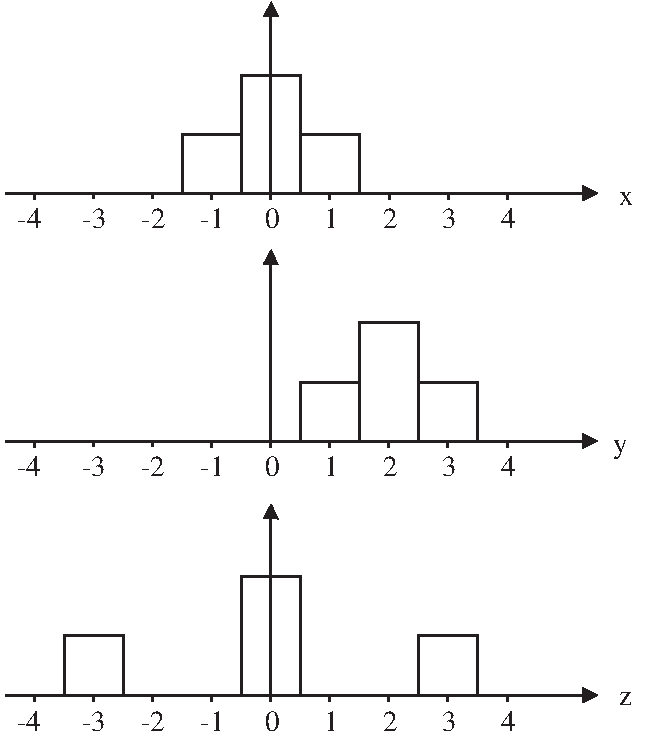
\includegraphics[scale=0.9]{figurer/fig5_3.pdf}
\caption{Histogrammer for $X$, $Y$ og $Z$}
	\label{fig:histXYZ}
\end{figure}

\noindent Sammenlignet med fordelingen til $X$, ser vi at fordelingen til
$Y$ har en annen forventning men samme spredning, mens
fordelingen til $Z$ har samme forventning men større spredning.
Litt løst kan vi si at et eventuelt mål for spredning i en
sannsynlighetsfordeling må ta sikte på å uttrykke et slags
``sannsynlig eller forventet avvik fra forventningsverdien''. La
oss gjøre noen betraktninger i denne forbindelse:

Forventningen $EX$ til en stokastisk variabel $X$ blir ofte
betegnet med $\mu_X$ eller kortere $\mu$ dersom det er klart
hvilken stokastisk variabel det dreier seg om. Av setning F4 i
forrige avsnitt følger nå at

\[        E (X - \mu ) = 0 \]

\noindent dvs. forventet avvik fra forventningsverdien (målt med fortegn)
er alltid null, og er således ubrukelig som spredningsmål. En
mulighet er nå å regne alle avvik positive, dvs. beregne tallverdien 
av avvikene og bruke

\[    E \mid X - \mu \mid   \]

\noindent som spredningsmål. Det viser seg imidlertid at dette
spredningsmål er matematisk lite bekvemt, og heller ikke særlig
fruktbart.
Følgende spredningsmål vil vise seg å være fruktbart:

\begin{center} \framebox[10cm]{\begin{minipage}{9cm}\rule{0cm}{0.5cm}
\begin{definisjon}
     Med {\em variansen} til en stokastisk
     variabel $X$ menes forventningen til $(X - \mu)^2$ hvor
     $\mu = EX$, og vi skriver
\[ \mbox{\ \ \ V1. \ \ \ \ } varX = E(X - \mu)^2 \] 
 \end{definisjon}  \vspace{-1.5\belowdisplayskip}
\end{minipage}} \end{center}

\noindent Dersom fordelingen til $X$ er godt sentrert om sin forventning
$\mu$ vil $(X - \mu)^2$ med stor sannsynlighet bli liten og
følgelig blir $E(X - \mu)^2$ liten. Omvendt, dersom fordelingen
er lite sentrert om forventningen, vil $(X - \mu)^2$ med stor
sannsynlighet bli stor og følgelig blir $E(X - \mu)^2$ stor.
Setter vi $\phi(X)=(X - \mu)^2$ og bruker setning F6, får vi
følgende beregningsformel for varians

\begin{center} \framebox[10cm]{\begin{minipage}{9cm}\rule{0cm}{0.5cm}
\[ \mbox{\ \ \ V2. \ \ \ \ }   varX = \sum_{x}{(x-\mu)}^2p(x) \]
\mbox{}  \end{minipage}} \end{center}

\noindent Av denne formelen går det fram at en varians alltid er et
ikke-negativt tall, og er null hvis og bare hvis den stokastiske
variable er en konstant (lik $\mu$).
I innledningseksemplet får vi $EX=EZ=0$ og $EY=2$, og følgelig

\[ \begin{array}{ccccc}
    varX&=&{(-1-0)}^2 \cdot \frac{1}{4}+{(0-0)}^2 \cdot \frac{1}{2}+
                   {(1-0)}^2 \cdot \frac{1}{4}&=&\frac{1}{2} \\
    varY&=&{(1-2)}^2 \cdot \frac{1}{4}+{(2-2)}^2 \cdot \frac{1}{2}+
                   {(3-2)}^2 \cdot \frac{1}{4}&=&\frac{1}{2} \\
    varZ&=&{(-3-0)}^2 \cdot \frac{1}{4}+{(0-0)}^2 \cdot \frac{1}{2}+
                   {(3-0)}^2 \cdot \frac{1}{4}&=&\frac{9}{2} 
\end{array} \]
Ved å kvadrere ut $(X - \mu)^2$ og bruke setningene om forventning,
kan vi få en alternativ formel for varians (merk at $\mu$ er en
konstant).
\begin{eqnarray*}
E(X - \mu)^2 &=&E(X^2-2 \mu X+{\mu}^2)=E(X^2)+E(-2 \mu X)+E({\mu}^2) \\
             &=&E(X^2)-2\mu EX+{\mu}^2=E(X^2)-2{\mu}^2+{\mu}^2 \\
             &=&E(X^2)-{\mu}^2
\end{eqnarray*}

\noindent Vi får derfor følgende setning

\begin{center} \framebox[10cm]{\begin{minipage}{9cm}
 \[ \mbox{\ \ \ V3. \ \ \ \ }varX = E(X^2) - (EX)^2 \]
\mbox{} \end{minipage}} \end{center}
\noindent som gir oss regneformelen

\begin{center} \framebox[10cm]{\begin{minipage}{9cm}
\[ \mbox{\ \ \ V4. \ \ \ \ }  varX = \sum_{x}x^2p(x)-{(EX)}^2 \]
\mbox{} \end{minipage}} \end{center}

\noindent I mange situasjoner er det lettere å beregne varians ved denne
formelen enn ved definisjonen.\\                    
                                                      
\begin{eksempel}{Et terningkast}
Vi har tidligere vist at forventningen til $X =$ antall øyne er
lik $EX=7/2$. Variansen til $X$ blir derfor
\begin{eqnarray*}
 varX&=&E{(X-\frac{7}{2})}^2= \\ &=& {(1-\frac{7}{2})}^2 \cdot
\frac{1}{6}+ {(2-\frac{7}{2})}^2 \cdot \frac{1}{6}+ \cdots
{(6-\frac{7}{2})}^2 \cdot \frac{1}{6}=\frac{35}{12}
\end{eqnarray*}
\noindent som alternativt kan beregnes ved
\begin{eqnarray*}
 varX&=&E(X^2)- {(\frac{7}{2})}^2 \\
 &=& 1^2 \cdot \frac{1}{6}+2^2 \cdot \frac{1}{6}
        + \cdots 6^2 \cdot \frac{1}{6}-{(\frac{7}{2})}^2=
   \frac{91}{6}-\frac{49}{4}=\frac{35}{12}
\end{eqnarray*}
\end{eksempel} 

\begin{eksempel}{To terningkast}
Vi har tidligere vist at forventningen til $S =$ sum øyne er lik
$ES=7$. Variansen til $S$ blir derfor
\begin{eqnarray*}
 varS&=&E{(S-7)}^2\\
 &=& {(2-7)}^2 \cdot \frac{1}{36}+{(3-7)}^2 \cdot \frac{2}{36}+ \cdots
           +{(12-7)}^2 \cdot \frac{1}{36}=\frac{35}{6}
\end{eqnarray*}

\noindent som alternativt kan beregnes slik
\begin{eqnarray*}
 varS&=&E(S^2)-{(7)}^2 \\
 &=& 2^2 \cdot \frac{1}{36}+3^2 \cdot \frac{2}{36}+ \cdots
            +{12}^2 \cdot \frac{1}{36}-7^2 =\frac{35}{6}
\end{eqnarray*}
\end{eksempel}
\begin{eksempel}{Tombola}
La situasjonen være som i Eksempel 9, hvor vi trakk et lodd
tilfeldig fra en tombola med $N$ lodder med verdier henholdsvis
$v_1, v_2, ..., v_N$. Vi husker at forventningen til $Y =$
verdien av det uttrukne lodd ble $EY=\bar{v}=\frac{1}{N}\sum_{i=1}^Nv_i$.
Variansen til $Y$ blir

\[   varY=E{(Y-\bar{v})}^2=\sum_{i=1}^N{(v_i-\bar{v})}^2 \cdot \frac{1}{N}=
                   \frac{1}{N} \sum_{i=1}^N{(v_i-\bar{v})}^2  \]
 
\noindent dvs. lik verdienes gjennomsnittlige kvadrerte avvik fra
gjennomsnittet.\footnote{Denne kvadratsum brukes ofte til å
karakterisere spredningen av observasjonene i et tallmateriale og
kalles da empirisk varians.}) Alternativt får vi

\[   varY=E(Y^2)-(EY)^2=\frac{1}{N}\sum_{i=1}^N{v_i}^2 -{(\bar{v})}^2. \]

\noindent Det siste uttrykket kan også fås ved å kvadrere ut 
	uttrykket ovenfor og summere (god øvelse, se også Oppgave~\ref*{kap:introduksjon}.11).
\end{eksempel}

\noindent Vi skal merke oss følgende setninger om varians:

\begin{center} \framebox[10cm]{\begin{minipage}{9cm}
\begin{eqnarray*}
 \mbox{ \ V5. \ \ \ \ } &  var(k)=0   \mbox{\ \  (k konstant)} \\
 \mbox{\ \ \ V6. \ \ \ \ } &      var(X+k)=var X \\
 \mbox{\ \ \ V7. \ \ \ \ } &    var(kX)=k^2 varX 
\end{eqnarray*} \mbox{} \end{minipage}} \end{center}
{\bf Begrunnelser :} Brukes setningene F3, F4 og F5 i forrige avsnitt, får vi
\begin{eqnarray*}
var (k)&=&E{(k-Ek)}^2=E{(k-k)}^2=E(0)=0 \\
var(X+k)&=&E{(X+k-E(X+k))}^2=E{(X+k-(EX+k))}^2 \\
        &=&E{(X-EX)}^2= varX \\
var(kX)&=&E{(kX-E(kX))}^2=E{(kX-kEX)}^2=E{(k(X-EX))}^2 \\
       &=&E(k^2{(X-EX)}^2)=k^2E{(X-EX)}^2=k^2 varX
\end{eqnarray*}

Vi vil også trenge en formel for variansen til en sum. Det er
kanskje grunn til å tro at $var(X+Y)$ er lik $var X+var Y$. Dette
er imidlertid generelt ikke tilfellet. Vi skal diskutere dette i
neste avsnitt.

Kvadratroten av $var X$ kalles {\em standardavviket} til $X$ og
betegnes ofte $\sigma (X)$, $\sigma_X$ eller kortere $\sigma$
dersom det er klart hvilken stokastisk variabel det er tale om,
altså

\[     \sigma=\sqrt{varX}  \]

\noindent Med denne skrivemåten blir altså ${\sigma}^2=varX$.
Det er klart
at begrepet standardavvik i og for seg er overflødig; kjenner vi
variansen, kjenner vi samtidig standardavviket og omvendt.
Standardavviket til $X$ har imidlertid den egenskap at det har
samme dimensjon som $X$ og $\mu =EX$, slik at spredningen målt
ved $\sigma$ kan avsettes på x-aksen (f. eks. i histogrammet) til
hver side av $\mu$ som et slags ``sannsynlige avvik''. 
Med de to alternative begrepene
varians og standardavvik oppnår vi også en større grad av
fleksibilitet, noen saksforhold kan uttrykkes mest oversiktlig
med varianser, andre med standardavvik.
La $X$ være en stokastisk variabel hvor $\mu =EX$ og
$\sigma^2=var X$. Da blir

\[ Z=\frac{X-\mu}{\sigma}  \]


\noindent kalt {\em den standardiserte variable til} $X$. Bruker vi
regnereglene for forventning og varians ser vi at

\[ EZ=E(\frac{X-\mu}{\sigma})=\frac{1}{\sigma}E(X-\mu)=
                                \frac{1}{\sigma}(EX-\mu)=0\]
\[  varZ=var(\frac{X-\mu}{\sigma})={(\frac{1}{\sigma})}^2var(X-\mu)
                =\frac{1}{{\sigma}^2}varX=1  \]

\noindent En standardisert variabel har altså alltid forventning null og
varians (og standardavvik) lik 1. Vi vil komme tilbake til bruken
av standardiserte variable i neste kapittel.
Begrepene forventning og varians vil komme til nytte senere i
Kapittel 6 i forbindelse med tilnærmet beregning av visse
sannsynligheter. Disse begreper spiller også en sentral rolle i
utviklingen av statistisk teori.



\section{Simultane fordelinger, uavhengighet og kovarians}

La $X$ og $Y$ være to stokastiske variable definert i forhold til
det samme utfallsrommet $\Omega$. Vi skal nå interessere oss for
begivenheter av typen

\[            (X=x)\cap (Y=y) \]

\noindent og spesielt sannsynlighetene for slike begivenheter.
     \footnote{Man pleier å kalle $(X,Y)$ for en
     stokastisk vektor, og $(x,y)$ en realisasjon av denne vektoren.}

\begin{center} \framebox[10cm]{\begin{minipage}{9cm}\rule{0cm}{0.5cm}
 \begin{definisjon}
     {\em Den simultane sannsynlighetsfordeling} til $X$ og $Y$
     er en oppregning av de mulige verdipar $(x,y)$ for $(X,Y)$ sammen med
     sannsynlighetene for at $(X,Y)$ antar disse verdipar.
     Den simultane sannsynlighetsfordeling for $X$ og $Y$ kan
     beskrives ved å angi funksjonen
        \[   p(x,y)=P((X=x)\cap (Y=y)) \]
     definert for de mulige verdipar $(x,y)$. Funksjonen $p(x,y)$ vil
    vi kalle {\em den simultane fordelingsfunksjonen} for $X$ og $Y$.
\end{definisjon}
\end{minipage}} \end{center}

\begin{eksempel}{Tre myntkast}
Betrakt de to stokastiske variable $X$ = antall sideskift og
 $Y$= antall kron, dvs.
\begin{center} \small
\begin{tabular}{cccccccccc}
$u$    &:& KKK & KKM & KMK & MKK & KMM & MKM & MMK & MMM \\
$X(u)$ &:&   0   &   1   &   2   &   1   &   1   &   2   &   1   &   0  \\
$Y(u)$ &:&   3   &   2   &   2   &   2   &   1   &   1   &   1   &   0
\end{tabular}
\end{center}
Her blir eksempelvis
\begin{eqnarray*}
     (X=0)\cap (Y=0)&=&\{\mbox{MMM}\} \\
     (X=0)\cap (Y=1)&=&\emptyset  \\
     (X=1)\cap (Y=1)&=&\{\mbox{KMM}, \mbox{MMK}\}
\end{eqnarray*}
Den simultane fordelingen for $X$ og $Y$ er da gitt ved tabellen:

\begin{center}
 \begin{tabular}{|c|cccc|c|} \hline
 $x\backslash y$ & 0 & 1 & 2 & 3 & Sum \\ \hline
 0 &1/8& 0 & 0 &1/8&2/8 \\
 1 & 0 &2/8&2/8& 0 &4/8 \\
 2 & 0 &1/8&1/8& 0 &2/8 \\ \hline
Sum&1/8&3/8&3/8&1/8& 1 \\ \hline
 \end{tabular}
\end{center}

\noindent For hvert tallpar $(x,y)$ viser tabellen $P((X=x)\cap (Y=y))$.
Ved å summere hver linje i tabellen får vi søylen til høyre.
Dette gir oss sannsynlighetsfordelingen til $X$. Ved å summere
hver søyle i tabellen får vi linjen nederst i tabellen. Dette gir
oss sannsynlighetsfordelingen til $Y$. Begge summeres til en.\\
\end{eksempel}
Når den simultane sannsynlighetsfordeling til $X$ og $Y$ er kjent,
kan vi beregne sannsynlighetsfordelingene til $X$ og $Y$ hver for
seg. Disse kalles nå {\em marginale fordelinger:}

La $y_1, y_2, ..., y_k$ være de mulige verdier av $Y$. Vi kan da
skrive
\begin{eqnarray*}
(X=x)&=&((X=x)\cap (Y=y_1))\cup ((X=x)\cap (Y=y_2))\cup \ldots \\
     & &     \mbox{\ \ \ \ \ \ } \cup ((X=x)\cap (Y=y_k)) 
\end{eqnarray*}
Siden denne unionen er disjunkt, får vi
\begin{eqnarray*}
 P(X=x)&=&P((X=x)\cap (Y=y_1))+P((X=x)\cap (Y=y_2))+\cdots \\
       & & \; \; \; \; \;+P((X=x)\cap (Y=y_k)) \\
       &=&p(x,y_1)+p(x,y_2)+\cdots +p(x,y_k)
\end{eqnarray*}
Betegner vi den marginale fordelingsfunksjonen til $X$ med
$p_1(x)$, får vi altså formelen

\[ p_1(x)=\sum_yp(x,y) \]

\noindent hvor summasjonen går over de mulige verdier av $Y$.
På tilsvarende måte, dersom vi betegner den marginale
fordelingsfunksjonen til $Y$ med $p_2(y)$, får vi formelen

\[ p_2(y)=\sum_xp(x,y) \]

\noindent hvor summasjonen går over de mulige verdier av $X$. Marginale
forde\-lingsfunksjoner kan altså utledes fra den simultane
fordelingsfunksjon ved å ``summere bort'' den andre variablen (se
Eksempel 20).

Det er ofte aktuelt å studere simultane fordelinger til mer enn
to stokastiske variable:
Med den {\em simultane fordelingsfunksjon} til $X_1, X_2, ...,
X_n$ menes funksjonen

\[ p(x_1, x_2, ..., x_n)=P((X_1=x_1)\cap (X_2=x_2)\cap ...\cap
                                                 (X_n=x_n)) \]

\noindent Resultatene ovenfor kan generaliseres, dvs. marginale
sannsynligheter finnes av simultane sannsynligheter
ved å ``summere bort'' de andre variablene.

\begin{center} \framebox[10cm]{\begin{minipage}{9cm}\rule{0cm}{0.5cm}
 \begin{definisjon}
     Dersom begivenhetene $(X=x)$ og $(Y=y)$
     er uavhengige, dvs.
     \[P ((X=x)\cap (Y=y))=P(X=x)\cdot P(Y=y), \]
     for alle mulige verdipar $(x,y)$, sier vi at $X$ og $Y$ er
     {\em uavhengige stokastiske variable}.
 \end{definisjon}
\end{minipage}} \end{center}
Av definisjonen følger at $X$ og $Y$ er uavhengige hvis og bare
hvis

\[     p(x,y)=p_1(x)\cdot p_2(y)   \]

\noindent dvs. den simultane fordelingsfunksjon er lik produktet av de
marginale. Vi ser at i Eksempel 16 er $X$ og $Y$ uavhengige, mens
i Eksempel 20 er $X$ og $Y$ ikke uavhengige, dvs. avhengige. Mer
generelt sier vi at $X_1, X_2, ..., X_n$ er {\em uavhengige
stokastiske variable} dersom

\[  p(x_1, x_2, ..., x_n)=p_1(x_1)p_2(x_2)\cdots p_n(x_n) \]

\noindent hvor $p_i(x_i)$ betegner den marginale fordelingsfunksjon til
$X_i$. Begrepet uavhengighet blir som oftest brukt konstruktivt i
den forstand at når man kjenner de marginale
fordelingsfunksjonene til $X_1, X_2, ..., X_n$ og er villig til å
anta at at $X_1, X_2, ..., X_n$ er uavhengige stokastiske
variable, så er den simultane fordelingsfunksjonen gitt ved
formelen ovenfor. \\

\begin{eksempel}{Solgt kvantum}
Et firma antar at solgt kvantum pr. dag ved et av sine to utsalg
er en stokastisk variabel $X$ med sannsynlighetsfordeling

\begin{center}
 \begin{tabular}{c|ccc}
 $x$ & 0 & 1 & 2 \\ \hline
 $P(X=x)$ & 0.6 & 0.3 & 0.1
 \end{tabular} \end{center}

\noindent For senere bruk beregner vi $EX=0.5$ og $varX=0.45$. Solgt
kvantum pr. dag ved det andre utsalget antas å være en stokastisk
variabel $Y$ med samme sannsynlighetsfordeling som $X$. Antas
uavhengighet blir den simultane fordeling for $(X, Y)$:

\begin{center}
 \begin{tabular}{|c|ccc|c|} \hline
 $x\backslash y$ & 0 & 1 & 2 & Sum \\ \hline
  0  & 0.36 & 0.18 & 0.06 & 0.6 \\
  1  & 0.18 & 0.09 & 0.03 & 0.3 \\
  2  & 0.06 & 0.03 & 0.01 & 0.1 \\ \hline
 Sum & 0.6 & 0.3 & 0.1 & 1.0  \\ \hline
 \end{tabular} \end{center}

\noindent dvs. hver sannsynlighet inne i tabellen er beregnet som produktet
av de respektive marginale sannsynligheter. Ut fra dette kan vi
bl. a. finne sannsynlighetsfordelingen til samlet solgt kvantum
$S=X+Y$. Vi får

\begin{center}
 \begin{tabular}{c|ccccc}
 $s$ & 0 & 1 & 2 & 3 & 4 \\ \hline
 $P(S=s)$&0.36&0.36&0.21&0.06&0.01
 \end{tabular} \end{center}

\noindent Diskuter antakelsen om uavhengighet!
\end{eksempel}

Anta at $X$ og $Y$ er to stokastiske variable med simultan
fordelingsfunksjon $p(x,y)$. La oss studere en ny stokastisk
variabel $Z$ avledet av $X$ og $Y$ ved at $Z=\phi (X,Y)$. Vi
ønsker å beregne $EZ=E\phi (X,Y)$. Nå er det klart at $EZ=\sum
zP(Z=z)$, hvor summasjonen går over alle mulige verdier av $Z$.
For å beregne $EZ$ etter denne formelen trenger vi imidlertid å
kjenne sannsynlighetsfordelingen til $Z$. I noen situasjoner er
det lett å finne denne fordelingen ut fra kjennskapet til den
simultane fordeling til $X$ og $Y$. Som regel kommer vi raskere
fram til svaret ved å bruke følgende formel

\begin{center} \framebox[10cm]{\begin{minipage}{9cm}\rule{0cm}{0.5cm}
\[ \mbox{\ \ \ F10. \ \ \ \ } E\phi(X,Y)=\sum_{(x,y)}\phi (x,y)p(x,y) \]
hvor summasjonen går over de mulige verdipar $(x,y)$. \\
  \end{minipage}} \end{center}

\noindent Begrunnelsen er analog med den for formel F6: Bruk definisjonen
av forventning for den avledede variable, og grupper så sammen
alle utfall som gir samme verdipar $(x,y)$. Vi ser at for å beregne 
forventningen til $Z=\phi (X,Y)$ er det nok å kjenne den simultane
fordeling til $X$ og $Y$: For alle mulige verdipar $(x,y)$ beregnes verdien
$\phi (x,y)$ som veies med sannsynligheten $p(x,y)$ hvoretter resultatene
summeres.

Formelen ovenfor kan nyttes til å gi et alternativt bevis for
setningen om forventningen til en sum (Oppgave~28). Vi kan nå også
vise et annet viktig resultat, nemlig

\begin{center} \framebox[10.5cm]{\begin{minipage}{9.5cm}
\[ \mbox{\ \ F11. \ \ \ } E(X\cdot Y)=EX\cdot EY
 \mbox{\ \ såframt $X$ og $Y$ er uavhengige.} \]
\mbox{}  \end{minipage}} \end{center}
{\bf Begrunnelse :} Vi bruker F10 med $\phi (X,Y)=X\cdot Y$, og bruker
uavhengigheten:
 
\begin{eqnarray*}
 E(X \cdot Y)&=&\sum_{(x,y)}xy \cdot p(x,y)=\sum_{(x,y)}xy \cdot p_1(x)p_2(y)\\
  &=& \sum_y \sum_x xy \cdot p_1(x)p_2(y)= \sum_y yp_2(y)(\sum_x xp_1(x)) \\
          &=&(\sum_x xp_1(x))(\sum_y yp_1(y))=EX \cdot EY
\end{eqnarray*}

\noindent Det må understrekes at ved avhengighet er det ikke tilfelle at
forventningen til et produkt er lik produktet av forventningene.\\

\begin{eksempel}{Kjøp - salg}
Et firma supplerer sitt lager av en bestemt reservedel ved
bestilling (fra utlandet) en gang hvert halvår. Antall enheter
$X$ som må bestilles neste gang betraktes som en stokastisk
variabel med forventning $EX=2.5$. Prisen pr. enhet på
bestillingstidspunktet er også en stokastisk variabel $Y$ med
forventning $EY=2000$ (i kroner). Utgiften ved neste bestilling
blir $Z=X\cdot Y$. Her er det rimelig å anta at $X$ og $Y$ er
uavhengige, slik at forventet utgift blir $EZ=EX\cdot EY=2.5\cdot
2000=5000$. Anta at det isteden dreier seg om solgt kvantum $X$
av en artikkel og $Y$ er markedspris slik at $Z=X\cdot Y$ er
salgsinntekten. Dersom en ønsker å beregne forventet salgsinntekt,
er det ikke uten videre rimelig å anta at salget er uavhengig av
markedspris, og da kan formel F11 ikke benyttes.
\end{eksempel}

Vi husker at variansen til en stokastisk variabel $X$ kunne
oppfattes som et mål for spredning eller variasjon. I det
følgende vil vi også trenge et mål for samvariasjon mellom to
stokastiske variable $X$ og $Y$. Følgende begrep viser seg å være
fruktbart:

\begin{center} \framebox[10cm]{\begin{minipage}{9cm}\rule{0cm}{0.5cm}
 \begin{definisjon}
     Med {\em kovariansen} mellom to stokastiske variable $X$ og $Y$ menes

\[ \mbox{\ \ \ C1. \ \ \ \ }  cov(X,Y)=E((X-EX)(Y-EY))   \]

Dersom  $cov(X,Y)=0$, sier vi at $X$ og $Y$ er {\em ukorrelerte.}
 \end{definisjon}
\end{minipage}} \end{center}
La oss gi en motivering for denne definisjonen: Dersom den
simultane sannsynlighetsfordeling til $(X,Y)$ er slik at store
(små) verdier av $X$ hører sammen med store (små) verdier av $Y$,
vil produktet $(X-EX)\cdot (Y-EY)$ bli positivt med stor
sannsynlighet. Følgelig blir forventningen av dette produktet
positivt, og dermed blir kovariansen mellom $X$ og $Y$ positiv.
Omvendt dersom små (store) verdier av $X$ gjennomgående hører
sammen med store (små) verdier av $Y$ vil produktet $(X-EX)\cdot(Y-EY)$
 bli negativt med stor sannsynlighet. Følgelig blir
forventningen negativ, og dermed blir kovariansen mellom $X$ og
$Y$ negativ. Dersom det er liten grad av samvariasjon mellom $X$
og $Y$ så blir kovariansen omkring null. Vi vil finne en
alternativ formel for kovarians. Betrakt

\[ (X-EX)(Y-EY)=X\cdot Y-X\cdot EY-Y\cdot EX+EX\cdot EY \]

\noindent Tar vi forventningen på begge sider får vi, siden
 $EX$, $EY$ og $EX\cdot EY$ er konstanter, at

\[ E(X-EX)(Y-EY)=E(X\cdot Y)-EX\cdot EY-EX\cdot EY+EX\cdot EY ,\]

\noindent Vi har derfor
\begin{center} \framebox[10cm]{\begin{minipage}{9cm}
\[ \mbox{\ \ \ C2. \ \ \ \ } cov(X,Y)=E(X\cdot Y)-EX\cdot EY   \]
\mbox{} \end{minipage}} \end{center}
\noindent som gir oss følgende beregningsformel

\begin{center} \framebox[10cm]{\begin{minipage}{9cm}
\[ \mbox{\ \ \ C3. \ \ \ \ } cov(X,Y)=\sum_{(x,y)}xy \cdot p(x,y)-EX\cdot EY \]
\mbox{}\end{minipage}} \end{center}

\noindent Ofte er det lettere å bruke denne formelen ved beregning av
kovarians enn definisjonen. Dersom $X$ og $Y$ er uavhengige
stokastiske variable husker vi at $E(X\cdot Y)=EX \cdot EY$. Innsettes
dette i C2 ser vi at i dette tilfellet blir $cov(X,Y)=0$. Vi har
derfor vist at

\begin{center} \framebox[10cm]{\begin{minipage}{9cm}
\[ \mbox{\ \ \ C4. \ \ \ \ }p(x,y)=p_1(x)\cdot p_2(y)
                               \mbox{ medfører } cov(X,Y)=0  \]
\mbox{}\end{minipage}} \end{center}

\noindent dvs. uavhengighet medfører ukorrelerthet. At det omvendte ikke
nødven\-dig\-vis er tilfelle viser bl. a. Eksempel 20 der vi finner
at kovariansen mellom $X$ og $Y$ er null, men variablene er
likevel avhengige.\\

\begin{eksempel}{Solgt kvantum}
For situasjonen i Eksempel 21 blir kovariansen mellom de solgte
kvanta $X$ og $Y$ pga. uavhengigheten lik null. Anta istedenfor
uavhengighet at den simultane fordeling for $X$ og $Y$ er gitt
ved

\begin{center}
 \begin{tabular}{|c|ccc|c|} \hline                                       
 $x\backslash y$ & 0 & 1 & 2 & Sum \\ \hline
  0  & 0.40 & 0.16 & 0.04 & 0.6 \\
  1  & 0.16 & 0.10 & 0.04 & 0.3 \\
  2  & 0.04 & 0.04 & 0.02 & 0.1 \\ \hline
 Sum & 0.6 & 0.3 & 0.1 & 1.0  \\ \hline
 \end{tabular} \end{center}

\noindent Vi ser at de marginale fordelingene er de samme som i Eksempel
21, og vi husker at

\[    EX=EY=0.5 \mbox{\ \ \ \ } varX=varY=0.45  \]

\noindent I dette tilfellet er det imidlertid positiv samvariasjon mellom
$X$ og $Y$. Vi har nemlig

\[ E(X\cdot Y)=0\cdot 0\cdot 0.40+0\cdot 1\cdot 0.16+\cdots +2\cdot
                                        2\cdot 0.02=0.34 \]

\noindent og ifølge C2 blir da $cov(X,Y)=0.34-0.5\cdot 0.5=0.09$, dvs.
positiv. Anta at den simultane fordeling for $X$ og$Y$ isteden er
gitt ved

\begin{center}
 \begin{tabular}{|c|ccc|c|} \hline
 $x\backslash y$ & 0 & 1 & 2 & Sum \\ \hline
  0  & 0.33 & 0.19 & 0.08 & 0.6 \\
  1  & 0.19 & 0.09 & 0.02 & 0.3 \\
  2  & 0.08 & 0.02 & 0.00 & 0.1 \\ \hline
 Sum & 0.6 & 0.3 & 0.1 & 1.0 \\ \hline
 \end{tabular} \end{center}

\noindent Nå er samvariasjonen negativ, og beregning av kovariansen gir
$cov(X,Y)=-0.08$. For ytterligere diskusjon se Oppgave~30.
\end{eksempel}

Nå er tiden inne for å presentere formelen for variansen til en
sum:

\begin{center} \framebox[10cm]{\begin{minipage}{9cm}
\[ \mbox{\ \ \ V8. \ \ \ \ }var(X+Y)=varX+varY+2cov(X,Y) \]
\mbox{}\end{minipage}} \end{center}
\noindent {\bf Begrunnelse :} Av definisjonen på varians følger at
\begin{eqnarray*}
var(X+Y)&=&E((X+Y)-E(X+Y))^2=E((X-EX)+(Y-EY))^2 \\
         &=&E((X-EX)^2+(Y-EY)^2+2(X-EX)(Y-EY)) \\
         &=&E(X-EX)^2+E(Y-EY)^2+2E((X-EX)(Y-EY))
\end{eqnarray*}
\noindent hvor vi har benyttet de kjente regnereglene for forventning.

     Av formelen ovenfor kan vi trekke en viktig konklusjon
\begin{center} \framebox[10cm]{\begin{minipage}{9cm}
\[ \mbox{V9. \ }  var(X+Y)=varX+varY
              \mbox{ når $X$ og $Y$ er ukorrelerte} \]
\mbox{} \end{minipage}} \end{center}
\noindent dvs. ukorrelerthet (og derfor spesielt uavhengighet) medfører at
variansen til en sum er lik summen av variansene. \\

\begin{eksempel}{To terningkast}
Med den tidligere benyttede modell er det klart at $X=$ antall
øyne i første kast og $Y=$ antall øyne i annet kast er uavhengige
stokastiske variable. Vi husker (se Eksempel 16) at
$varX=varY=35/12$. Følgelig blir variansen til $S=$ sum øyne

\[ varS=var(X+Y)=varX+varY=\frac{35}{12}+\frac{35}{12}=\frac{35}{6} \]

\noindent som stemmer med det vi fant med betydelig mer regnearbeid i
Eksempel 17.
\end{eksempel}

Formel V8. kan generaliseres (Oppgave~34).

\begin{center} \framebox[10cm]{\begin{minipage}{9cm}
\[ \mbox{\ \ \ V10. \ \ \ \ } var(\sum_{i=1}^n X_i)= \sum_{i=1}^n var(X_i)
             + \sum_{i \ne j}cov(X_i,X_j)   \]
\mbox{} \end{minipage}} \end{center}

\noindent dvs. variansen til en sum er lik summen av variansene pluss
summen av alle mulige par av kovarianser. Merk at siden
$cov(X_1, X_2)=cov(X_2, X_1)$ etc., vil to og to av disse
kovariansene være like. Vi merker oss at

\begin{center} \framebox[10cm]{\begin{minipage}{9cm}
\[ \mbox{V11. \ } var(\sum_{i=1}^n X_i)= \sum_{i=1}^n var(X_i)
             \mbox{\ \ såframt \ } cov(X_i,X_j)=0   \]
\mbox{}\end{minipage}} \end{center}

\noindent Denne formelen gjelder spesielt når $X_1, X_2, ..., X_n$ er
uavhengige.

Kovarians som mål for samvariasjon lider av den svakhet at det
er avhengig av måleenhetene for variablene, f.eks.\ om et beløp
er målt i kroner eller øre. Dette unngår vi ved å bruke 
{\em korrelasjonskoeffisienten} definert ved
\begin{center} \framebox[10cm]{\begin{minipage}{9cm}
\[  \mbox{C5.\ \ \ \ \ } \rho (X,Y)=\frac{cov(X,Y)}{\sqrt{varX} \cdot \sqrt{varY}} \]
\mbox{}\end{minipage}} \end{center}
Korrelasjonskoeffisienten har egenskapen
\[     -1\leq \rho (X,Y)\leq +1.      \]
Dette er det modellteoretiske motstykke til den empiriske
korrelasjonskoef\-fisienten definert i Kapittel 1 og begrepene knyttes
sammen i Kapittel 9.

\section{Betingede sannsynlighetsfordelinger}

La $(X,Y)$ ha simultan fordelingsfunksjon

\[   p(x,y)=P((X=x)\cap (Y=y))\]

\noindent og la de marginale fordelingsfunksjonene være henholdsvis


\[     p_1(x)=P(X=x) \mbox{\ \ og \ \   } p_2(y)=P(Y=y). \]

\noindent La nå $x$ være slik at $p_1(x)>0$, og la oss beregne
 betingede sannsynligheter gitt at $X=x$. Vi får

\[ P(Y=y \mid X=x)=\frac{P((X=x)\cap (Y=y))}{P(X=x)}=\frac{p(x,y)}{p_1(x)} \]

\noindent Dette blir kalt {\em den betingede sannsynlighetsfordeling for
$Y$ gitt $X=x$.} På tilsvarende måte blir, når $p_2(y)>0$

\[ P(X=x \mid Y=y)=\frac{P((X=x)\cap (Y=y))}{P(Y=y)}=\frac{p(x,y)}{p_2(y)} \]

\noindent kalt {\em den betingede sannsynlighetsfordeling for $X$ gitt $Y=y$}.
Betingede sannsynlighetsfordelinger har samme egenskaper som
vanlige sannsynlighetsfordelinger (Oppgave~37). Forventningen til
$Y$ beregnet i den betingede fordeling gitt $X=x$ skriver vi

\[            E(Y\mid X=x)   \]
og kaller {\em den betingede forventning} for $Y$ gitt $X=x$. På
tilsvarende måte betyr $E(X\mid Y=y)$ den betingede forventning
for $X$ gitt $Y=y$. \\

\begin{eksempel}{Betinget forventning}
Anta at $(X,Y)$ har simultan fordeling som i Eksempel 20. Da blir
den betingede fordeling for $Y$ gitt $X=1$

\begin{center}
 \begin{tabular}{c|cccc}
 $y$& 0 & 1 & 2 & 3 \\ \hline
 $P(Y=y \mid X=1)$& 0 &1/2&1/2&0
 \end{tabular}
\end{center}
\noindent mens den betingede fordeling for $X$ gitt $Y=1$ er
\begin{center}
 \begin{tabular}{c|ccc}
 $x$& 0 & 1 & 2  \\ \hline
 $P(X=x \mid Y=1)$& 0 &2/3&1/3
 \end{tabular}
\end{center}
\noindent Vi ser at $E(Y\mid X=1)=3/2$, mens $E(X\mid Y=1)=4/3$
\end{eksempel}
                                                          
Det er lett å vise (Oppgave~37) at $X$ og $Y$ er uavhengige hvis
og bare hvis den betingede fordeling for $Y$ gitt $X=x$ er lik
den marginale fordeling for $Y$ for alle verdier av x.

                    

\section{$\star$Mer om forventning}
\small
Vi vil avslutte dette kapitlet med å presentere en del
supplerende stoff om sannsynlighetsfordelinger og forventning. Vi
vil gi noen eksempler på anvendelser av teorien ovenfor, samtidig
som vi gjør noen spredte betraktninger over emner som kan øke vår
teoretiske innsikt. Disse er, i rekkefølge, konvolusjon,
setningen om dobbeltforventning, prediksjon med kvadratisk tap,
muligheten for at en forventning er uendelig, samt St. Petersburg
spillet. \\

\begin{eksempel}{Samlet etterspørsel}
En vare etterspørres av tre kunder, og daglig etterspurt kvantum
fra disse oppfattes som tre stokastiske variable $X_1$, $X_2$ og
$X_3$. Disse antas å være uavhengige med samme
sannsynlighetsfordeling gitt ved
\begin{center}
 \begin{tabular}{c|cccc}
 $x$& 0  & 1 & 2 & 3 \\ \hline
 $P(X=x)$ & 0.4 & 0.3 & 0.2 & 0.1
\end{tabular}
\end{center}
\noindent Vi ser at $EX=0\cdot 0.4+1\cdot 0.3+2\cdot 0.2+3\cdot 0.1=1.0$.
Samlet daglig etterspørsel etter varen blir

\[ S=X_1+X_2+X_3. \]

\noindent Vi ønsker å finne sannsynlighetsfordelingen til $S$. Den viser
seg å bli
\begin{center} \small \addtolength{\tabcolsep}{-0.4\tabcolsep}
 \begin{tabular}{c|cccccccccc}
 $s$& 0  & 1 & 2 & 3 & 4 & 5 & 6 & 7 & 8 & 9 \\ \hline
 $P(S=s)$ &0.064&0.144&0.204&0.219&0.174&0.111&0.056&0.021&0.006&0.001
\end{tabular}
\end{center}
\noindent Vi ser eksempelvis at
\begin{eqnarray*}
    P(S\geq 6)&=&P(S=6)+P(S=7)+P(S=8)+P(S=9) \\
              &=&0.056+0.021+0.006+0.001=0.084.
\end{eqnarray*}
\noindent Forventningen til $S$ blir

\[ ES=0\cdot 0.064+1\cdot 0.144+2\cdot 0.204+\cdots +9\cdot 0.001=3.0 \]

\noindent men dette følger enklere av at

\[ ES=EX_1+EX_2+EX_3=1.0+1.0+1.0=3.0. \]

\noindent Utledning av sannsynlighetsfordelingen:
\begin{center}
\begin{tabular}{cll}
 $(S=0)$ & inntreffer på en måte:   &  0+0+0 \\
 $(S=1)$ & inntreffer på tre måter: &  0+0+1, 0+1+0, 1+0+0 \\
 $(S=2)$ & inntreffer på seks måter:&  0+0+2, 0+2+0, 2+0+0 \\
       &                                    &  0+1+1, 1+0+1, 1+1+0 \\
 $(S=3)$ & inntreffer på ti måter:  &  0+0+3, 0+3+0, 3+0+0 \\
      &                                     & 0+1+2, 1+0+2, 2+0+1 \\
      &                                     & 0+2+1, 1+2+0, 2+1+0 \\
      &                                     & 1+1+1              \\
   \vdots &                                 &                     \\  
 $(S=9)$& inntreffer på en måte:    & 3+3+3.
\end{tabular}
\end{center}
\noindent Eksempelvis blir (legg merke til hvor vi bruker antakelsen om
uavhengighet)

\begin{eqnarray*}
     P(S=1)&=&P((X_1=0)\cap (X_2=0)\cap (X_3=1)) \\
           &+&P((X_1=0)\cap (X_2=1)\cap (X_3=0))\\
           &+&P((X_1=1)\cap (X_2=0)\cap (X_3=0)) \\
           &=&P(X_1=0)\cdot P(X_2=0)\cdot P(X_3=1) \\
           &+&P(X_1=0)\cdot P(X_2=1)\cdot P(X_3=0) \\
           &+&P(X_1=1)\cdot P(X_2=0)\cdot P(X_3=0) \\
           &=&3\cdot 0.4^2\cdot 0.3=0.144.
\end{eqnarray*}

\noindent Det overlates til leseren å verifisere de andre tallene i
tabellen. Selv om dette var et relativt enkelt eksempel, ser vi
at det medfører et betydelig regnearbeid.
\end{eksempel}

Problemer som dreier seg om summer av uavhengige stokastiske
variable med samme sannsynlighetsfordeling dukker opp i mange
anvendelser, og er blitt tatt opp på prinsipielt grunnlag under
betegnelsen {\em konvolusjon}. Det er utviklet spesielle
teknikker for å løse slike problemer, men det vil føre for langt
å komme inn på disse her.
En type problemer av en litt annen karakter enn forrige eksempel
har vi i det følgende.\\



\begin{eksempel}{Etterspørsel i leveringstiden}
La $X$ være daglig etterspørsel etter en vare. Anta at $X$ har
sannsynlighetsfordeling gitt ved
\begin{center}
 \begin{tabular}{c|cccc}
 $x$& 0  & 1 & 2 & 3 \\ \hline
 $P(X=x)$ & 0.4 & 0.3 & 0.2 & 0.1
\end{tabular}
\end{center}
\noindent Vi ser at forventet daglig etterspørsel er

\[ EX=0\cdot0.4+1\cdot 0.3+2\cdot0.2+3\cdot 0.1=1. \]

\noindent Anta at etterspørselen på suksessive dager
 $X_1, X_2, X_3, \ldots$
kan oppfattes som uavhengige stokastiske variable med samme
sannsynlighetsfordeling som $X$. Anta videre at leveringstiden
ved bestilling av varen er en stokastisk variabel $N$ som antar
verdier blant de naturlige tall, som er uavhengig av $X_i$'ene og
med sannsynlighetsfordeling
\begin{center}
 \begin{tabular}{c|ccc}
 $n$& 1 & 2 & 3 \\ \hline
 $P(N=n)$ & 0.25 & 0.50 & 0.25
\end{tabular}
\end{center}
\noindent La $S_N$ være etterspørselen i leveringstiden. Da er

\[ S_N=X_1+\cdots +X_N . \]

\noindent Her vil antall ledd i summen være stokastisk, i motsetning til i
Eksempel 26. Vi ønsker å finne sannsynlighetsfordelingen til
$S_N$. Den viser seg å bli

\begin{center} \small \addtolength{\tabcolsep}{-0.4\tabcolsep}
 \begin{tabular}{c|cccccccccc}
 $s$& 0  & 1 & 2 & 3 & 4 & 5 & 6 & 7 & 8 & 9 \\ \hline
 $P(S=s)$ &0.196&0.231&0.226&0.180&0.094&0.048&0.019&0.005&0.001&0.000
\end{tabular}
\end{center}
\noindent Vi ser eksempelvis at
\begin{eqnarray*}
P(S_N\geq 5) &=& P(S_N=5) + \cdots + P(S_N=9) \\
             &=&0.048 + 0.019 + 0.005 + 0.001 + 0.000 = 0.073.
\end{eqnarray*}
\noindent Forventningen til $S_N$ blir (dersom vi bruker alle desimalene)

\[ES_N = 0\cdot 0.196 + 1\cdot 0.231 + 2\cdot 0.226 + \cdots +
                                    9\cdot 0.000 = 2.0. \]
\noindent Vi ser at $ES_N=EN\cdot EX$, og vi skal vise nedenfor av dette
generelt er tilfelle i slike situasjoner det her er tale om.
En begrunnelse for sannsynlighetsfordelingen ovenfor krever, med
de teknikker vi har til rådighet her, betydelig regnearbeid. De
ulike sannsynlighetene kan finnes ved å betinge med hensyn på
lengden av leveringstiden, eksempelvis (legg merke til hvor vi
bruker antakelsene om uavhengighet)

\begin{eqnarray*}
P(S_N=2)&=&P(N=1)P(S_N=2 \mid N=1)+P(N=2)P(S_N=2 \mid N=2) \\
        & &+P(N=3)P(S_N=2 \mid N=3) \\
        &=&\frac{1}{4}P(X_1=2)+\frac{1}{2}P(X_1+X_2=2)+
                    \frac{1}{4}P(X_1+X_2+X_3=2) 
\end{eqnarray*}
\noindent Ifølge opplysningene er $P(X_1=2)=0.2$, mens
\begin{eqnarray*}
P(X_1+X_2=2) &=&P((X_1=0)\cap (X_2=2)) \\
             &+&P((X_1=2)\cap (X_2=0)) \\
             &+&P((X_1=1)\cap (X_2=1)) \\
             &=&P(X_1=0)\cdot P(X_2=2)  \\
             &+&P(X_1=2)\cdot P(X_2=0) \\
             &+&P(X_1=1)\cdot P(X_2=1) \\
             &=&2\cdot 0.4\cdot 0.2 + 0.3\cdot 0.3 = 0.25
\end{eqnarray*}
\noindent På tilsvarende måte finner vi (se også Eksempel 26)

\[ P(X_1 + X_2 + X_3 = 2) = 0.204. \]

\noindent Innsatt ovenfor gir dette

\[ P(S_N=2)=\frac{1}{4}\cdot 0.2+\frac{1}{2}\cdot 0.25+
                                   \frac{1}{4}\cdot 0.204=0.226 \]

\noindent Det overlates til leseren å verifisere de andre sannsynlighetene
i tabellen ovenfor.
\end{eksempel}

Situasjonen ovenfor er et eksempel på en såkalt {\em
forgreningsprosess}. Slike problemstillinger dukker opp i mange
anvendelser, og det er derfor utviklet generelle teorier for
analyse av slike, noe som det vil føre for langt å komme inn på
her.

Vi vil nå presentere {\em setningen om dobbeltforventning} som kan
være et nyttig hjelpemiddel i mange anvendelser:
La $X$ og $Y$ være to stokastiske variable med simultan
sannsynlighetsfordeling $p(x,y)=P((X=x)\cap (Y=y))$. Vi kan da
beregne $E(Y\mid X=x)$. Denne forventning vil generelt være en
funksjon av $x$, vi skriver

\[ \phi (x)=E(Y\mid X=x). \]

\noindent Betrakt den stokastiske variable $\phi (X)$. Denne stokastiske
variable blir ofte betegnet $E(Y\mid X)$. La oss studere
forventningen til denne variable.
\begin{eqnarray*}
E\phi (X)&=&\sum_x \phi(x)p_1(x)=\sum_x E(Y \mid X=x)p_1(x) \\
         &=&\sum_x (\sum_y yp_2(y\mid x))p_1(x)=\sum_x \sum_y yp(x,y) \\
         &=&\sum_y y \sum_x p(x,y) = \sum_y yp_2(y)=EY
\end{eqnarray*}
\noindent der $p_2(y\mid x)$ er den betingede fordeling for $Y$ gitt $X=x$.
Vi har dermed vist at
\begin{center} \framebox[10cm]{\begin{minipage}{9cm}
\[ \mbox{\ \ F12.\ \ \ \ \ } EE(Y\mid X)=EY  \]
\mbox{} \vspace{-0.5\belowdisplayskip}  \end{minipage}} \end{center}

\noindent og det er dette som kalles setningen om dobbeltforventning.
Forventningen til $Y$ kan altså beregnes som en veid sum over $x$
av $E(Y\mid X=x)$ med vekter lik sannsynlighetene for at $X=x$. I
praksis kan setningen om dobbeltforventningen utnyttes på
følgende måte:

I situasjoner der forventningen $EY$ skal beregnes, men dette
ikke er lett å gjøre direkte, kan en ofte finne en egnet
stokastisk variabel $X$, beregne den betingede forventning av $Y$
gitt $X$, og så bruke regelen om dobbeltforventning. La oss se på
et par slike anvendelser : \\


\begin{eksempel}{Spedisjon}
Et vareparti skal sendes fra A til B med en av tre mulige
spedisjonsfirmaer nummerert 1, 2, og 3. Av erfaring vet man at
tiden det tar kan variere. La

     $X=$ nummer på det spedisjonsfirma som brukes. \\
\indent     $Y=$ tiden i døgn fra innlevering til mottak .

\noindent Anta at en vurderer situasjonen dithen at

\begin{center}
\begin{tabular}{c|ccc}
  $y$& 1 & 2 & 3 \\ \hline
 $P(Y=y \mid X=1)$&0.5&0.4&0.1 \\
 $P(Y=y \mid X=2)$&0.3&0.4&0.3 \\
 $P(Y=y \mid X=3)$&0.2&0.6&0.2 
\end{tabular}
\end{center}
\noindent Anta videre, basert på erfaring med pristilbud og service etc. at
det er like stor sjanse for at oppdraget blir gitt til firma nr.
1 som til de andre to tilsammen, mens de to andre firmaene er
like sannsynlige. Hva blir forventet leveringstid (før det er
fastlagt hvem oppdraget blir gitt til). Vi ser at

\[ E(Y\mid X=1)=1.6 \; \; E(Y\mid X=2)=2.0 \; \; E(Y\mid X=3)=2.0 \]

\noindent og bruker vi setningen om dobbeltforventning blir
\begin{eqnarray*}
E(Y) &=& E(Y\mid X=1)P(X=1)+E(Y\mid X=2)P(X=2) \\
     & & + E(Y\mid X=3)P(X=3) \\
     &=&1.6\cdot 0.50 + 2.0\cdot 0.25 + 2.0\cdot 0.25 = 1.8.
\end{eqnarray*}
\noindent Det overlates til leseren å vise at
\begin{center}
 \begin{tabular}{c|ccc}
 $y$& 1 & 2 & 3 \\ \hline
 $P(Y=y)$ & 0.375 & 0.450 & 0.175
\end{tabular}
\end{center}
\noindent slik at vi igjen kan finne

\[ EY=1\cdot 0.375 + 2\cdot 0.450 + 3\cdot 0.175 = 1.8. \]

\noindent I dette eksemplet er det nok omtrent det samme arbeid ved begge
utregningsmetoder, men det finnes eksempler der utregning uten
bruk av setningen om dobbeltforventning blir mye mer komplisert.
\end{eksempel}

En spesielt viktig anvendelse oppstår i følgende situasjon:
La $X_1, X_2, X_3, ...$ være stokastiske variable som alle har
samme forventning, kall den $EX$. La $n$ være gitt naturlig tall
og la

\[ S_n=X_1+X_2+ \cdots +X_n. \]
                                          
\noindent Av formel F8 følger at
\begin{center} \framebox[10cm]{\begin{minipage}{9cm}
\[ \mbox{\ \ \ F13. \ \ \ \ } ES_n=n\cdot EX.         \]
\mbox{} \vspace{-0.5\belowdisplayskip}  \end{minipage}} \end{center}
\noindent Anta nå at $N$ er en stokastisk variabel som antar verdier blant
de naturlige tall og som er uavhengige av $X_i$'ene. Betrakt

\[ S_N = X_1 + X_2 + \cdots + X_N. \]

\noindent Her er, i motsetning til $S_n$, antall ledd i summen stokastisk.
Følgende formel synes rimelig
\begin{center} \framebox[10cm]{\begin{minipage}{9cm}
\[ \mbox{\ \ \ F14. \ \ \ \ }ES_N = EN \cdot EX.   \]
\mbox{} \vspace{-0.5\belowdisplayskip}  \end{minipage}} \end{center}
\noindent {\bf Begrunnelse :} Vi ser at
    
\[ E(S_N\mid N=n)=E(S_n\mid N=n)=ES_n=nEX. \]

\noindent Nest siste likhet er en følge av at $N$ og $X_i$'ene er
uavhengige, og følgelig vil $S_n$ og $N$ være uavhengige. Vi har
derfor

\[ E(S_N\mid N)=NEX. \]

\noindent Ifølge setningen om om dobbeltforventning blir

\[ ES_N=E(E(S_N\mid N))=E(N\cdot EX)=EX\cdot EN \]

\noindent fordi $EX$ er en konstant som kan settes utenfor det ytterste
forventningstegnet.
Under forutsetningen av at $X_i$'ene er uavhengige stokastiske
variable med samme forventning og varians, finnes det også
regneformler for variansen til summer av typen ovenfor. I
tilfellet med sum med et gitt antall ledd
\begin{center} \framebox[10cm]{\begin{minipage}{9cm}
\[ \mbox{\ \ \ V12. \ \ \ \ }varS_n = n var X.   \]
\mbox{} \vspace{-0.5\belowdisplayskip}  \end{minipage}} \end{center}
\noindent I tilfellet med et stokastisk antall ledd
\begin{center} \framebox[10cm]{\begin{minipage}{9cm}
\[ \mbox{\ \ \ V13. \ \ \ \ } var S_N = EN\cdot var X + var N\cdot (EX)^2. \]
\mbox{} \vspace{-0.5\belowdisplayskip}  \end{minipage}} \end{center}
\noindent Det vil føre for langt å vise denne formel her.
Setning F14 og V13 kan blant annet nyttes til å finne
forventning og varians til etterspørsel i leveringstiden i
Eksempel 27 uten først å foreta omfattende beregninger for å
etablere sannsynlighetsfordelingen.
En annen anvendelse av setningen om dobbeltforventning er: \\


\begin{eksempel}{Ventetid til første kron}
La $N=$ ventetiden til første kron i myntkast.
En alternativ måte å beregne forventningen til $N$ på, er som
følger. La
\begin{eqnarray*}
     X&=&1 \mbox{\ \ dersom første kast er kron} \\
      &=&0 \mbox{\ \ dersom første kast er mynt.}
\end{eqnarray*}
\noindent Da blir
\begin{eqnarray*}
     EN&=&E(N\mid X=0)P(X=0)+E(N\mid X=1)P(X=1) \\
       &=&\frac{1}{2}(E(N\mid X=0)+E(N\mid X=1)).
\end{eqnarray*}
\noindent Men nå er
\begin{eqnarray*}
     E(N\mid X=0)&=&1+EN \\
     E(N\mid X=1)&=&1
\end{eqnarray*}
\noindent fordi forventet ventetid til kron, gitt første kast mynt, må
være lik en (det første kastet) pluss forventet ventetid fra dette
kast til første kron, som er $EN$. Vi får derfor

\[       EN=\frac{1}{2}(1+EN+1)=1+\frac{1}{2}EN \]

\noindent Løses denne ligning med hensyn på $EN$ ser vi at $EN = 2$.
\end{eksempel}

Vi vil nå se på et interessant aspekt ved begrepene forventning
og varians, nemlig {\em prediksjon med kvadratisk tapsfunksjon:}


Et eksperiment skal utføres. Eksperimentet medfører bl. a. at en
stokastisk variabel $Y$ antar en bestemt verdi $y$. Anta at
sannsynlighetsfordelingen $P(Y=y)$ til $Y$ er kjent, slik at $EY$
og $varY$ også er kjent. La $\mu =EY$. La oss tenke oss at vi,
før eksperimentet blir utført, blir bedt om å tippe hvilken verdi
på $Y$ vi kommer til å observere. La oss anta kvadratisk tap,
dvs. dersom vi tipper verdien $z$ og observerer verdien $y$, så
taper vi beløpet $(y-z)^2$. Før eksperimentet er utført kan vi
oppfatte tapet som en stokastisk variabel $T=(Y-z)^2$ og
forventet tap blir

\[ ET=E(Y-z)^2. \]

\noindent Vi ønsker å velge $z$ slik at vi minimerer forventet tap. Det
viser seg at da må vi velge $z=\mu$ og forventet tap er da lik
$varY$. For å innse dette vil vi omforme uttrykket for forventet
tap.
\begin{eqnarray*}
     E(Y-z)^2&=&E(Y-\mu +\mu -z)^2 \\
             &=&E((Y-\mu )^2+2(Y-\mu )(\mu -z)+(\mu -z)^2) \\
             &=&E(Y-\mu )^2+2(\mu -z)E(Y-\mu )+E(\mu -z)^2.
\end{eqnarray*}
\noindent Vi har først trukket fra og lagt til $\mu$, deretter kvadrert ut
uttrykket og brukt regnereglene for forventning. I det siste
uttrykket er det først leddet lik variansen, mens det midterste
leddet er lik null. Vi får

\[ E(Y-z)^2=varY+(\mu -z)^2\]

\noindent og vi ser at dette er større enn eller lik $varY$, med likhet
hvis og bare hvis $z$ velges lik $\mu$.

Anta nå at vi kan observere en stokastisk variabel $X$ som gir
delvis informasjon om $Y$, f.eks. ved at den simultane
fordeling til $X$ og $Y$, $P((X=x)\cap (Y=y))$ er kjent. Dersom vi
får vite at $X=x$, vil det være den betingede fordeling for $Y$
gitt $X=x$ som er relevant for oss når vi skal foreta
prediksjonen. Med kvadratisk tap vil det være optimalt å
predikere forventningen i denne betingede fordelingen, dvs. at vi
gir prediksjonen $Z=E(Y\mid X=x)$. Forventet tap blir da
variansen i den betingede fordelingen. \\


\begin{eksempel}{Uendelig forventning}
La $X$ være en stokastisk variabel som antar verdier blant de
naturlige tall. Anta at sannsynligheten for at $X$ antar verdien
$x$ er omvendt proporsjonal med kvadratet av verdien $x$, dvs. at
$X$ har punktsannsynlighet av form

\[ p(x)=P(X=x)=k \cdot \frac{1}{x^2} \; \; x=1,2, \ldots   \]

\noindent der $k$ er en konstant slik at $ \sum p(x)=1$. \footnote{Lesere
med gode kunnskaper i matematisk analyse vil lett kunne finne ut at
$k= 6/{\pi}^2$.})

\noindent Forventningen til $X$ blir

\[  EX=\sum_{x=1}^{\infty}xp(x)=k \sum_{x=1}^{\infty}x \frac{1}{x^2}=
            k \sum_{x=1}^{\infty} \frac{1}{x}=\infty \]

\noindent Summen representerer ikke noe endelig tall, den er uendelig.
\end{eksempel}

Dette eksemplet har lært oss at dersom en stokastisk variabel $X$
kan anta et uendelig antall verdier, er det mulig at forventningen
til $X$ ikke eksisterer som noe endelig tall. Dette betyr bl.a.
at man i enkelte setninger for forventning må ta reservasjon om
at de forventninger som inngår eksisterer, dersom setningen også
skal gjelde i situasjoner med uendelig antall mulige verdier.
Eksempelvis, for at setningen $E(X+Y)=EX+EY$ skal gjelde i slike
situasjoner, må vi anta at $EX$ og $EY$ eksisterer, bl. a. for å
unngå uttrykk av form $\infty - \infty$ som er en meningsløshet.

     Vi går videre til \\


\begin{eksempel}{Petersburg spillet}
Et kasino tilbyr et spill hvor spilleren for en innsats på $k$
kroner får knipse en mynt inntil første kron inntreffer. Dersom
spilleren får første kron i n'te omgang utbetales $2^n$ kroner
til spilleren.  Lar vi $N=$ ventetid til
første kron, vil altså gevinsten være en stokastisk variabel

\[   G=2^N-k. \]

\noindent Siden sannsynlighetsfordelingen til $N$ er gitt ved

\[ p(x)={(\frac{1}{2})}^n \; \; n=1,2, \ldots \]

\noindent vil forventet gevinst bli (bruk formel F6)

\begin{eqnarray*}
 EG&=& \sum_{n=1}^{\infty}(2^n-k)p(n)= 
         \sum_{n=1}^{\infty}(2^n-k){(\frac{1}{2})}^n \\
   &=&-k+(1+1+1+ \cdots )= \infty
\end{eqnarray*}
\noindent Vi ser at forventningen til $G$ ikke eksisterer som noe endelig
tall. Dette innebærer bl. a. at det ikke finnes noen innsats $k$,
samme hvor stor den er, som gjør dette spillet til rettferdig
spill i den forstand vi studerte i Eksempel 13. $(EG=0)$.
Analysen ovenfor forutsetter egentlig at kasinoet har uendelige
ressurser (og spilleren uendelig med tid til rådighet). La oss
tenke oss at spillets regler er slik at spilleren kan spille
inntil 20 omganger for innsatsen. Det meste kasinoet risikerer å
utbetale etter et spill er derfor $2^{20}$=1 048 476 kroner. Nå
er

\[ G=\left\{ \begin{array}{ll}
              2^N-k & \mbox{\ for \ } N \leq 20 \\
              2^{20}-k & \mbox{\ for \ } N > 20 
             \end{array} \right. \]
\noindent Forventet gevinst blir nå isteden

\begin{eqnarray*}
 EG&=& \sum_{n=1}^{20}(2^n-k)p(n)+(2^{20}-k)P(N>20) \\ 
   &=& \sum_{n=1}^{20}(2^n-k){(\frac{1}{2})}^n+
               (2^{20}-k)(1-\sum_{n=1}^{20}{(\frac{1}{2})}^n) \\
   &=&-k+21  
\end{eqnarray*}

\noindent slik at 21 kroner vil være den innsats som gjør spillet
rettferdig. I et kasino med store ressurser er det altså
mulig å etablere rettferdige spill med mulighet for å gjøre en
formue selv med en beskjeden innsats, men merk at sannsynligheten
for moderat (selv positiv) gevinst blir relativt liten. Dette og
andre eksempler viser at forventningsverdi ikke i alle
situasjoner kan brukes som et mål for verdien av et spill for en
spiller, evt. verdien av et investeringsobjekt for en investor.
For eksempel vil de færreste være villige til å satse
et stort beløp dersom sjansen for å mangedoble dette er liten,
f. eks. investere 10 000 kroner med sjanse på 1/10 000 for å få
tilbake 1 milliard selv om forventet gevinst her er 90 000
kroner.
\end{eksempel}
\normalsize

\section{Oppgaver}
\small
\begin{enumerate}
\item En modell og to stokastiske variable $X$ og $Y$ er gitt i
     tabellen
     \begin{center}
     \begin{tabular}{c|cccccc}
     $u$&$u_1$&$u_2$&$u_3$&$u_4$&$u_5$&$u_6$ \\ \hline
     $P(u)$&$\frac{1}{8}$&$\frac{1}{8}$&$\frac{2}{8}$&$\frac{2}{8}$
                            &$\frac{1}{8}$&$\frac{1}{8}$ \\
     $X(u)$&0&0&1&2&3&4 \\
     $Y(u)$&1&2&$-1$&1&$-2$&0
     \end{tabular}
     \end{center}   
     Finn sannsynlighetsfordelingene til henholdsvis $X$ og $Y$.
     Finn også sannsynlighetsfordelingene til følgende
     stokastiske variable $X+Y, X-Y, X^2, Y^2$ og $X^2 + Y^2$.

\item En modell og to stokastiske variable $X$ og $Y$ er gitt i
     tabellen
     \begin{center}
     \begin{tabular}{c|ccccc}
     $u$&$u_1$&$u_2$&$u_3$&$u_4$&$u_5$ \\ \hline
     $P(u)$&$\frac{1}{8}$&$\frac{1}{8}$&$\frac{1}{8}$&$\frac{2}{8}$
                            &$\frac{3}{8}$ \\
     $X(u)$&1&2&2&1&4 \\
     $Y(u)$&4&4&4&2&1
     \end{tabular}
     \end{center}   
     Vis at $X$ og $Y$ har samme sannsynlighetsfordeling. Følger
     det herav at $S=X+Y$ og $V=X+X=2X$ har samme
     sannsynlighetsfordeling?

\item Regn ut forventningen til de stokastiske variable som er
     omtalt i Oppgave~1 og~2, både ut fra definisjonen av
     forventning og ut fra de respektive
     sannsynlighetsfordelinger. Der det er mulig illustrerer også
     hvordan de etablerte regneregler for forventning kan nyttes
     for å forenkle regnearbeidet.

\item Tegn histogrammer for de stokastiske variable omtalt i Oppgave~1 og~2.

\item Kast en terning 100 ganger og observer antall øyne i hvert
     kast, og beregn gjennomsnittlig antall øyne i de 100
     kastene. Sammenlikn dette med forventet antall øyne i et
     kast 7/2.

\item For en falsk terning har man funnet ut at det er rimelig å
     sette sannsynligheten for 1, 2, 3, 4, 5 og 6 øyne lik
     henholdsvis 0.19, 0.17, 0.17, 0.17, 0.17 og 0.13. (se
	Oppgave~\ref*{kap:diskrete}.8). La $X$ være antall øyne i et kast. Beregn $EX$
     og $varX$.

\item La antall øyne i første og annet kast med terningen i
     forrige oppgave være henholdsvis $X$ og $Y$, og la $S=X+Y$
     være sum øyne. Finn sannsynlighetsfordelingen til $S$ og
     beregn ut fra denne $ES$ og $varS$. Kunne disse størrelsene
     ha vært funnet på en enklere måte?

\item Det utføres tre myntkast med en rettferdig mynt. La $X$ være
     antall kron. Finn sannsynlighetsfordelingen til $X$, og
     beregn $EX$ og $varX$.          

\item La situasjonen være som i Oppgave~\ref*{kap:kombinatorikk}.15, og la $X$ være
     antall Bordauxviner som en deltaker får smake. Finn
     sannsynlighetsfordelingen til $X$ og beregn $EX$.

\item I Oppgave~\ref*{kap:kombinatorikk}.18 hva blir forventet antall rette?

\item La situasjonen være som i Oppgave~\ref*{kap:kombinatorikk}.19, og la $X$ være
     antall defekte i utvalget. Finn sannsynlighetsfordelingen
     til $X$ og beregn $EX$.

\item La situasjonen være som i Oppgave~\ref*{kap:kombinatorikk}.21, og la $X$ være
     antall funksjonærer i utvalget. Finn
     sannsynlighetsfordelingen til $X$ og beregn $EX$.

\item La situasjonen være som i Oppgave~\ref*{kap:betinget}.25, og la $X$ være
     antall ganger en ny arbeider lykkes i løpet av tre forsøk.
     Finn sannsynlighetsfordelingen til $X$ og beregn $EX$.
     Besvar denne oppgaven også under forutsetningene i Oppgave~\ref*{kap:betinget}.26.

\item La situasjonen være som i Oppgave~\ref*{kap:betinget}.29, og la $X$ være
     ventetiden til første justering. Finn
     sannsynlighetsfordelingen til $X$ og beregn $EX$. La $Y$
     være antall ekstra justeringer i løpet av uken. Finn
     sannsynlighetsfordelingen til $Y$ og beregn $EY$. Besvar
     denne oppgaven også under forutsetningene i Oppgave~\ref*{kap:betinget}.30.

\item La situasjonen være som i Oppgave~\ref*{kap:betinget}.31, og la $X$ være
     antall kvinner på kurs. Finn sannsynlighetsfordelingen til
     $X$ og beregn $EX$. La $Y$ være antall menn på kurs, og finn
     $EY$. Løs også oppgaven under de alternative trekningsmåtene
     som er angitt.

\item La situasjonen være som i Oppgave~\ref*{kap:betinget}.34, og la $X$ være
     antall rette tippetegn. Finn $EX$ og $varX$ under begge
     forutsetninger som er angitt.

\item En pakning inneholder 10 artikler, hvorav 3 er defekte. Det
     trekkes tilfeldig et utvalg på 4 artikler. La $X$ være
     antall defekte artikler i utvalget. Finn
     sannsynlighetsfordelingen til $X$. Beregn $EX$ og $varX$.

\item En produksjonsprosess gir defekt artikkel med sannsynlighet
     $p=0.05$. Det produseres 4 artikler. Anta uavhengighet. La
     $X$ være antall defekte artikler. Finn
     sannsynlighetsfordelingen til $X$. Beregn $EX$ og $varX$.

\item En pakning inneholder 5 artikler hvorav en er defekt. For å
     finne ut hvilken som er defekt trekkes tilfeldig artikler
     fra pakningen, og disse blir undersøkt en etter en. La $X$
     være antall artikler som må undersøkes. Finn
     sannsynlighetsfordelingen til $X$. Beregn $EX$ og $varX$.

\item $\star$Det utføres gjentatte terningkast med en rettferdig terning.
     La $X$ være antall kast som er nødvendig for at sum øyne
     skal være minst 6. Finn sannsynlighetsfordelingen til $X$.
     Beregn $EX$ og $varX$.

\item I et spill er innsatsen 1 krone hvoretter spilleren får rett
     til 3 terningkast. Dersom spilleren ikke får noen sekser, er
     innsatsen tapt. Dersom han får en sekser, får han 2 kroner
     tilbake (innsatsen + en krone), ved to seksere får han 4
     kroner tilbake og ved tre seksere får han 8 kroner. Er dette
     et rettferdig spill? Hvis ikke hvor stort beløp må spilleren
     få tilbake ved tre seksere for å gjøre spillet rettferdig.

\item La $X$ være antall kroner i tre myntkast. To spill er tilbudt
     \begin{itemize}
     \item[(a)]  gir utbetaling $Y=2X-2$ 
     \item[(b)]  gir utbetaling $Z=(X-1)^2$.
     \end{itemize}
     Hvilket spill vil du foretrekke?\\
     Lønner det seg å spille dersom innsatsen er 2 kroner?

\item Du triller terning og kan etter hvert kast velge om du vil stoppe og
      innkassere et kronebeløp lik sum øyne hittil. Haken er at straks du
      får en ener mister du alt. Når lønner det seg å stoppe?
      Hva er en rettferdig innsats for å få spille?


\item En bedrift har 8 ansatte som utfører et arbeid med en viss
     risiko for skade, og bedriften ønsker å tegne en forsikring
     på kr 100 000 pr ansatt. Sannsynligheten for at en arbeider
     blir skadet i løpet av et år vurderes til 0.0001. Hva er en
     ``rettferdig'' årspremie for bedriften (vi ser bort fra
     omkostninger, fortjeneste etc.).

\item La $Y\geq X$, dvs. $Y(u)\geq X(u)$ for alle $u$. Vis at da
     er $EY\geq EX$.

\item La $X$ være stokastisk variabel som antar verdiene $1, 2,\ldots N$,
      hver med sannsynlighet $1/N$. Finn $EX$ og $varX$.

\item La $X_1, X_2, \ldots X_n$ være uavhengige stokastiske
     variable, alle med samme forventning $\mu$ og samme varians
     ${\sigma}^2$. La
     \[ \bar{X}=\frac{1}{n} \sum_{i=1}^{n} X_i \]
      Vis at $E(\bar{X})=\mu $ og $var(\bar{X})={\sigma}^2/n$

\item Følgende gir god øvelse i å regne med forventning, varians
      og kovarians :
      \begin{itemize}
       \item[(a)]  Bruk F3, F4 og F5 til å vise at
          \[ E(a+bX)=a+bEX. \]
          Bruk F6 til å gi et alternativt bevis for denne formelen.
       \item[(b)]  Bruk V6 og V7 til å vise at
           \[ var(a+bX)=b^2varX. \]
       \item[(c)]  Vis at standardavviket har egenskapen
          \[ \sigma (a+bX)=\mid b\mid \sigma (X). \]
          der $\mid b\mid$ betegner tallverdien av $b$.
       \item[(d)]  Vis at kovarians har egenskapen
          \[ cov(a+bX, c+dY)=b\cdot d \cdot cov(X,Y). \]
     \end{itemize}

\item \begin{itemize}
       \item[(a)]  Bruk F10 til å vise at
          \[ E(bX+dY)=bEX+dEY. \]
       \item[(b)]  Vis at når $X$ og $Y$ er uavhengige så er
          \[ var(bX+dY)=b^2varX+d^2varY. \]
          Er formelen $var(X-Y)=varX-varY$ korrekt?
     \end{itemize}

\item  \begin{itemize}
      \item[(a)]  Vis at korrelasjonskoeffisienten $\rho (X,Y)$
          har egenskapen at for positive konstanter $b$ og $d$ er
          \[ \rho (a+bX, c+dY)=\rho (X,Y). \]
          Hva skjer dersom enten $b$ eller $d$ (eller begge) er negative? 
      \item[(b)]  Vis at korrelasjonskoeffisienten har egenskapen
          \[ -1\leq \rho (X,Y)\leq +1. \]
          Hint: Vis først at
          \[  var(bX+Y)=b^2varX+2b cov(X,Y)+varY. \]
          Gjør bruk av denne formel med $b=-cov(X,Y)/varX$.
      \item[(c)]  Hva kan sies om $X$ og $Y$ dersom \\
        (i)  $\rho (X,Y)=0$ \ \ (ii) $\rho (X,Y)=1$  (iii)\ \ $\rho (X,Y)=-1$.
        \item[(d)] Uttrykk formel V8 og V10 standardavvik og 
                   korrelasjonskoeffisienter.
     \end{itemize}

\item La situasjonen være som i Eksempel 23.
     \begin{itemize}
     \item[(a)]  Finn sannsynlighetsfordelingen til samlet solgt kvantum
          $S$ i hvert av tilfellene med positiv og negativ
        samvariasjon.
     \item[(b)]  Beregn variansen til $S$ i begge tilfeller direkte ut
          fra (a) og ved V8..
     \item[(c)]  Sammenlign (a) og (b) med tilfellet
          uavhengighet (Eksempel 21).
     \item[(d)]  Beregn korrelasjonskoeffisienten mellom $X$ og $Y$ i de
          tre tilfellene uavhengighet, positiv og negativ samvariasjon.
     \end{itemize}  

\item Finn følgende korrelasjonskoeffisienter
     \begin{itemize}
     \item[(a)]  mellom $X$ og $Y$ i Oppgave~1.
     \item[(b)]  mellom $X$ og $Y$ i Oppgave~2.
     \item[(c)]  mellom $X+Y$ og $X-Y$ i Oppgave~1.
     \end{itemize}  

\item Avkastingen pr. investert krone i hvert av to
     investeringsobjekter antas å være stokastiske variable med
     forventning og standardavvik gitt ved
     \begin{center}
      \begin{tabular}{lcc}
                                & Forventning &   Standardavvik\\
     Investering nr. 1 \ldots   &    0.10     &     0.08       \\
     Investering nr. 2 \dots    &    0.15     &     0.12
      \end{tabular}
     \end{center}
     En investor har bestemt seg for å plassere halvparten av sin
     kapital i hvert av objektene. Finn forventning og
     standardavvik til avkasting pr. investert krone dersom
     korrelasjonskoeffisienten mellom avkastingene i hvert av
     objektene er
     \begin{center}
      \begin{tabular}{ccc}
          (i) 0   &    (ii) 0.5   &    (iii) $-$0.5
      \end{tabular} 
     \end{center}
     Formuler problemstillingen generelt og diskuter mulige
     konsekvenser for investering under usikkerhet.

\item Et firma har to bilselgere A og B. Antall solgte biler pr.
     uke for de to antas å være uavhengige stokastiske variable
     $X$ og $Y$ med sannsynlighetsfordeling henholdsvis
     \begin{center}
     \begin{tabular}{c|cccccc|ccc}
      $x$& 0 & 1 & 2 & & &$y$& 0 & 1 & 2  \\ \cline{1-4} \cline{7-10}
      $P(X=x)$&0.3&0.4&0.3& & &$P(Y=y)$&0.5&0.4&0.1
     \end{tabular}
     \end{center}
     \begin{itemize}
     \item[(a)]  Finn den simultane fordeling til $X$ og $Y$.
     \item[(b)]  Finn sannsynligheten for at de en uke selger like mange
          biler.
     \item[(c)]  Finn sannsynlighetsfordelingen til $S=X+Y$.
     \item[(d)]  Gitt at det en uke ble solgt to biler. Hva er
     sannsynligheten for at A solgte begge?
     \end{itemize}

\item 
     \begin{itemize}
      \item[(a)]  Vis formel V10 i teksten, dvs.

         \[  var(\sum_{i=1}^n X_i)= \sum_{i=1}^n var(X_i) +
                                        \sum_{i \ne j}cov(X_i,X_j)   \]
     \item[(b)]  Vis at
         \[  cov(\sum_{i=1}^n X_i,\sum_{j=1}^m Y_j)= 
                     \sum_{i=1}^n \sum_{j=1}^m cov(X_i,Y_j)   \]
     \end{itemize}
\item 
      \begin{itemize}
      \item[$\star$(a)]  Kan $X$ og $X^2$ være uavhengige?
      \item[(b)]  Kan $X$ og $X^2$ være ukorrelerte?
      \item[(c)]  Vis at dersom $X$ og $Y$ er uavhengige så er også
          $U=f(X)$ og $V=g(Y)$ uavhengige.
     \end{itemize}

\item 
      \begin{itemize}
        \item[(a)]  Vis at betingede sannsynlighetsfordelinger har samme
          egenskaper som vanlige sannsynlighetsfordelinger (se
          Kapittel 5.2).
      \item[(b)]  Vis at $X$ og $Y$ er uavhengige hvis og bare hvis den
          betingede fordeling for $Y$ gitt $X=x$ er lik den
          marginale fordeling for $Y$.
     \end{itemize}

\item Finn den kumulative fordeling til følgende stokastiske
     variable
      \begin{itemize}
     \item[(a)]  Antall øyne $X$ i et myntkast.
     \item[(b)]  Antall kron $X$ i to myntkast.
     \item[(c)]  Sum øyne $S$ i to terningkast.
     \item[(d)]  De stokastiske variable $X$ og $Y$ i Oppgave~1.
     \item[(e)]  De stokastiske variable $X, Y, S$ og $V$ i Oppgave~2.
     \end{itemize}
     Tegn figurer for å illustrere disse kumulative fordelingene.


\item $\star$Fordelingen til en stokastisk variabel $X$ sies å være
     {\em symmetrisk} om $a$ dersom
 \[    P(X=a+x)=P(X=a-x) \mbox{ for alle $x$.} \]
     Vis at dersom dette er tilfelle, så må
 \[     EX=a  \mbox{\ \ \ (såframt forventningen eksisterer).}\]
     Hint: Vis først at $X-a$ og $a-X$ må ha samme fordeling og
     følgelig samme forventning.

\item 
    \begin{itemize}
    \item[$\star$(a)]  Vis at $E(X^2)\geq (EX)^2$.
    \item[(b)]  La $X$ ha fordelingen
     \begin{center}
     \begin{tabular}{c|cc}
      $x$&$a/A$ &$b/B$  \\ \hline
      $P(X=x)$&$A/(A+B)$ &$B/(A+B)$
     \end{tabular}
     \end{center}
      der a, b, A og B er positive tall. \\
      Bruk resultatet i (a) til å vise ulikheten
      \[  \frac{{(a+b)}^2}{A+B} \leq \frac{a^2}{A}+ \frac{b^2}{B} \]
      Denne ulikheten kan generaliseres til
      \[  \frac{{(a+b+c+ \ldots)}^2}{A+B+C+ \ldots} \leq 
                \frac{a^2}{A}+ \frac{b^2}{B} + \frac{c^2}{C}+ \ldots \]
      og har flere anvendelser, bl.a. i Kapittel 14.
     \end{itemize}

\item $\star$La $X_1$, $X_2$ og $X_3$ være uavhengige med samme
     sannsynlighetsfordeling $p(x)$.
    \begin{itemize}
    \item[(a)]  Finn sannsynlighetsfordelingen til $S=X_1+X_2$ dersom
          $p(x)$ er gitt ved
    \begin{center}
    \begin{tabular}{cc|ccccccc|ccc}
        & $x$& 0 & 1 & 2 & & & &$x$& 0 & 1 & 2\\ \cline{2-5} \cline{9-12}
     (i)&$P(X=x)$&$\frac{1}{3}$&$\frac{1}{3}$&$\frac{1}{3}$& & &
    (ii)&$P(X=x)$&$\frac{2}{5}$&$\frac{1}{5}$&$\frac{2}{5}$
   \end{tabular}
    \begin{tabular}{cc|ccc}
        & $x$& 0 & 1 & 2 \\ \cline{2-5}
     (iii)&$P(X=x)$&$\frac{3}{6}$&$\frac{2}{6}$&$\frac{1}{6}$
   \end{tabular}           
   \end{center}
          Hint: Gå fram som i Eksempel 25.
    \item[(b)]  Finn sannsynlighetsfordelingen til $T=X_1+X_2+X_3$ i
       tilfellene (i), (ii) og (iii).
    \item[(c)]  Tegn histogrammer og kommenter disse (se også Kapittel
          6.5 om normaltilnærming).
     \end{itemize}

\item
    \begin{itemize}
     \item[(a)]  Kast en terning gjentatte ganger og observer antall
      øyne. Tegn et empirisk histogram etter \\
          (i) $n=20$ kast \ \  (ii) $n=100$ kast.
     \item[(b)]  Kast to terninger gjentatte ganger og observer sum
          øyne. Tegn et empirisk histogram etter \\
          (i) $n=20$ kast \ \  (ii) $n=100$ kast.
     \item[(c)]  Kast tre terninger gjentatte ganger og observer sum
          øyne. Tegn et empirisk histogram etter\\
          (i) $n=20$ kast \ \  (ii) $n=100$ kast.
     Kommenter resultatene.
     \end{itemize}
     Denne oppgaven gjøres enklest ved å simulere terningkast på PC.
\end{enumerate}

\normalsize

